\documentclass[12pt]{article}
%%%%%%%%%%%%%%%%%%%%%%%%%%%%%%%%%%%%%%%%
\usepackage{amsmath}
\usepackage{verbatim}
\usepackage[usenames,dvipsnames]{color}
\usepackage{setspace}
\usepackage{lscape}
\usepackage{longtable}
\usepackage[top=1.25in,bottom=1.25in,left=1in,right=1in]{geometry}
\usepackage{graphicx}
\usepackage{epstopdf}
\usepackage{epsfig}
\usepackage{fancyhdr}
\usepackage{booktabs}
\usepackage{dcolumn}
\usepackage{arydshln}
\usepackage{natbib}
\usepackage{tabularx}
\usepackage{subfigure}

{\newcommand{\districts}{  28,475}
{\newcommand{\provinces}{   2,282}
{\newcommand{\countries}{     151}

\newtheorem{proposition}{Proposition}
\newtheorem{corollary}{Corollary}

\setcounter{MaxMatrixCols}{10}
\newcolumntype{d}[1]{D{.}{.}{-2.#1}}
\newenvironment{proof}[1][Proof]{\noindent\textbf{#1.} }{\ \rule{0.5em}{0.5em}}
\setlength{\columnsep}{.2in}
%\psset{unit=1cm}

\newcolumntype{R}{>{\raggedleft\arraybackslash}X}

%\def\sym#1{\ifmmode^{#1}\else\(^{#1}\)\fi}

\begin{document}
\begin{titlepage}
\vspace{2in} \noindent {\large \today}

\vspace{.5in} \noindent {\Large \textbf{\strut The role of land in temperate and tropical agriculture}}

\vspace{.25in} \noindent {\large T. Ryan Johnson}

\vspace{.05in} \noindent Washington University

\vspace{.25in} \noindent {\large Dietrich Vollrath}

\vspace{.05in} \noindent University of Houston

\vfill \noindent \textsc{Abstract} \hrulefill

\vspace{.05in} \noindent We document differences in the elasticity of agricultural output with respect to land in temperate and tropical regions. We estimate this elasticity from the relationship of rural labor/land ratios and agro-climatic constraints using global district-level data. We find the elasticity in temperate areas (0.285) is higher than the tropics (0.126), and this is not an artifact of the level of development. The land elasticity influences the degree of decreasing returns to labor and capital in agriculture, and thus how sensitive living standards are to shocks in productivity and population. Evidence from the post-war mortality transition supports this prediction.
 
\vspace{.1in} \hrule

\vspace{.5in} \noindent {\small JEL Codes: O1, O13, O44, Q10}

\vspace{.1in} \noindent {\small Keywords: land constraints, land elasticity, agricultural productivity, agro-climatic, temperate, tropical}

\vspace{.1in} \noindent {\small Contact information: 201C McElhinney Hall, U. of Houston, Houston, TX 77204, devollrath@uh.edu. We thank Tasso Adamopoulos, Francesco Caselli, Areendam Chanda, Martin Fiszbein, Oded Galor, Remi Jedwab, Nippe Lagerl{\"o}f, Debin Ma, Stelios Michalopolous, Nathan Nunn, {\"O}mer {\"O}zak, Stephen Smith, Enrico Spolaore, Joachim Voth, and David Weil, as well as seminar participants at LSU, York University, London School of Economics, Texas A\&M Ag. Econ, the Brown Conference on Deep-rooted Determinants of Development, George Washington University, and the University of Houston brown bag series for their comments. This paper previously circulated under the title ``How Tight are Malthusian Constraints?''. All errors remain our own.}
\end{titlepage}

\pagebreak 

\section{Introduction}
\doublespacing 
Agricultural production relies on the use of a finite (or inelastically supplied) resource, land. But that reliance on land need not be identical in different locations. To be specific, the elasticity of agricultural output with respect to land may differ by climate or the type of crops suitable for production. This land elasticity is relevant to any study of growth and development that includes an agricultural sector, as with the mild assumption of constant returns to scale, one minus the land elasticity tells us how sensitive agricultural output is to the use of non-land inputs like capital and labor. This in turn determines how many non-land inputs move out of (or into) agriculture in response to shocks to productivity and population. Differences in the land elasticity by crop or climate thus imply differences in the reaction of economies to shocks, with implications for studies of comparative development, structural change, Malthusian stagnation, the take-off to sustained growth, and long-run growth with finite resources.\footnote{Agriculture and land feature in stories of divergence across global regions \citep{kp2001,galor2008trading,vollrath2011,vv08,vv13,cs2015}. On structural change, see \cite{Gollin:2007oq,Restuccia:2008hc,weilwilde2009,Gollin:2010ys,ev2016clim}. For Malthusian stagnation, see \cite{ashraf2010dynamics} for a baseline model, and \citet{Galor:2011uq} for a review of major contributions to the literature on the take-off to growth \citep{gw00,galor2002natural,Hansen:2002fk,doepke2004accounting,cs2005,lagerlof2006,craftsmills2009,strulik2008population}. On the relevance of resources for long-run growth, see \cite{perettovalente2015}.} 

In this paper, we estimate the land elasticity, and show that it varies across different agricultural regions and climate types. Estimating the parameter(s) of an agricultural production function is not straightforward, for the standard reasons that total factor productivity and some inputs may be unobserved. To address these issues, we first develop a method for estimating the aggregate land elasticity using the relationship between the labor/land ratio in agriculture and the potential agro-climatic yield across small geographic units (e.g. 2nd-level districts within states/provinces). The methodology relies on the mobility of labor between districts within states, as well as between agricultral and non-agricultural uses. We show that this mobility is supported in the data, first by reviewing recent research on this subject, second by providing evidence drawn from the Demographic and Health Surveys, and third by documenting the small size (in terms of population and area) of districts.

Given mobility, our method does not require us to identify exactly what the inputs are beyond land and labor, avoiding mis-measurement issues. We use agro-climatic yield data to give us a source of exogenous variation in productivity, and combine that with measures of district-level development (e.g. night lights, road density, and urbanization) to control for other unobservable elements of agricultural productivity. Most relevant, our estimates are made using only within-state variation across districts, meaning that unobservable variation in productivity across states, as well as across countries, is excluded from the estimates. This means our framework is robust to arbitrary distortions (e.g. taxes, subsidies) of agricultural and factor prices at the state level.

We assemble data at the district level for rural labor/land ratios in the year 2000, and combine that with a measure of potential agro-climatic yield in districts built from the data of \citet{galorozak2016}. As in their work, our measure is built on constraints plausibly unaffected by human activity (e.g. soil quality and length of growing season) from the Global Agro-Ecological Zone (GAEZ) project \citep{gaez}, combined with information on the calorie content of various crops. Grid cell potential caloric yields are aggregated to the district level to serve as our measure of agro-climatic yield.\footnote{There are two studies that also study the spatial distribution of labor at the global level in some capacity. The first is \citet{mfm2014}, who examine the growth of urbanization at the grid-cell level over the last two-thousand years. The second is \citet{hssw2016}, who examine the spatial distribution of economic activity at the grid-cell level using night lights.}

In the end, we have a dataset of\districts \ districts, coming from\provinces \ states in\countries \ countries. We then divide districts into ``temperate'' and ``tropical'' regions based on their agro-climatic characteristics. In our baseline we make this division based on the types of crops that can be grown within a district. The temperate region includes districts that can grow crops such as wheat, barley, and rye, while the tropical region includes districts that can grow crops such as paddy rice, cassava, and pearl millet. We also divide districts based on their frost-free days (e.g. tropical areas are frost-free all year round, while temperate areas are not), or by their K{\"o}ppen-Geiger climate classification \citep{kottek2006}, and our results are similar. Regardless of the definition, our assignment is made at the district level and we do not assume that agriculture has a homogenous land elasticity within a country. 

Our baseline estimate is that the land elasticity is 0.285 in temperate districts. In contrast, our baseline estimate of the land elasticity is only 0.126 for tropical districts. The difference is statistically significant, and is robust to the exclusion of districts that contain large urban areas, districts that are large relative to their state, or of districts from any developed country. Further, the results are consistent if we use alternative measures of rural labor/land ratios, alternative measures of the potential agro-climatic yield, or alternative measures of the area of agricultural land used within a district. In all cases, the aggregate land elasticity in temperate districts is approximately 0.16 higher than in tropical districts, and the difference is statistically significant.\footnote{These results are consistent with the work of \citet{Ruthenberg:1976zr} and \citet{bray1994}, who discuss the inherent differences in the response of tropical crops (rice, in particular) to the application of labor. They both cite the relatively \textit{high} elasticity of output with respect to labor in tropical agriculture, which is consistent with a low elasticity of output with respect to land.} As the measure of agro-climatic yield we use is based on staple crops, our results should be interpreted as differences in the land elasticity in staple crop production.\footnote{We show as part of our robustness checks that our results hold if districts that are large livestock or cash crop producers are included or excluded from the regressions. The Appendix also contains explicit estimates of the land elasticity for districts that are major cash crop producers, and their elasticites tend to be slightly higher than the tropical value, save for tea producers which have an elasticity near the temperate estimate.}

Relative to the existing literature, our approach to estimating the aggregate land elasticity has several advantages. The standard approach has been to use country-level panel data \citep{Hayami:1970ly,Hayami:1985cr,cpr1997,mm2001,Mundlak:2000dq,mbl2012,et2013mango} to estimate agricultural production functions, with a common set of coefficients across countries for each input, including land. Issues arise with unobserved productivity, the measurement of non-land inputs, and the assumption that coefficients are common to all countries. Some have examined heterogeneity in these coefficients \citep{gg2003,Wiebe2003Resource-Qualit} by continent, while others have attempted to estimate country-level coefficients using factor analysis to address unobserved productivity \citep{et2013mango,ev2016clim}. Compared to this, our district-level data allows us to control for unobserved country and state-level effects, and the use of agro-climatic yield data gives us an explicit measure of productivity.\footnote{Firm-level methods \citep{olleypakes1996,levpetrin2003} are not applicable in our context because we do not have a panel of district data, nor do we have full data on the inputs used at the district level.} 

As may be apparent, we are not estimating the elasticity of a \textit{farm}-level production function, but rather an \textit{aggregate} production function. Farm-level estimates of the land elasticity would not necessarily be informative about the aggregate production function, given that those estimates would refer to farmers using a given technique, while the aggregate function can be thought of as an envelope across techniques available to farmers \citep{Hayami:1970ly}.\footnote{More general treatments of this idea can be found in \citet{houthakker1955} and \citet{jones2005}. In short, the farm-level land elasticities may not be informative on the aggregate land elasticity, and farm-level production functions may well take on different forms (i.e. Leontief verus Cobb-Dougals) than the aggregate function.} The aggregate land elasticity is a useful parameter for studying the role of the agricultural sector and its interaction with other sectors at the macro level, as we discuss below, while farm-level elasticities would be useful for studying farm-level policies or outcomes within the agricultural sector itself. This distinction explains one of the limitations of our study, which is that we cannot use our results to identify why the aggregate land elasticity differs between temperate and tropical regions. An explanation would require details on the interaction of farmers with biological production functions for specific crops that are beyond the scope of this paper. 

With that caveat in mind, we show in the second half of the paper that the aggregate land elasticity is central to any study that looks at the relationship of agriculture to non-agriculture, and the variation we have identified between temperate and tropical regions has implications for development. The intuition is that the land elasticity dictates, given an assumption of constant returns to scale, the degree of decreasing returns to scale for labor and capital in agriculture. A large land elasticity implies more severe decreasing returns, and in response to shocks to productivity or population this means more severe movements of those factors into or out of agriculture. Temperate areas therefore have exaggerated responses to shocks relative to tropical areas. This is a benefit to temperate areas when shocks are positive (e.g. higher TFP or lower population growth), but a burden in the face of negative shocks (e.g. lower TFP or higher population growth).

In the last part of the paper we confirm these predictions by using data from \cite{aj07} to examine the consequence of population shocks arising from the epidemiological transition after World War II. The shock to mortality was negatively correlated with GDP per capita, and GDP per worker, across all developing countries. But we find that the size of that negative correlation was three times larger for countries with temperate land elasticities compared to countries with tropical land elasticities, consistent with our intuition. The difference in correlation is statistically significant, and holds whether we measure the population shock in terms of mortality or life expectancy.

At a broader level, variation in the land elasticity may be relevant for the study of historical and contemporary development. For any given positive shock to productivity (or negative shock to population growth), areas with temperate land elasticities experience more urbanization and faster growth in living standards, whatever the fundamental driver of those shocks: institutions, geography, or culture.\footnote{It would be hopeless to summarize or cite all the research on comparative development. Several useful reviews of this literature can be found in \cite{ajr2005handbook,nunn_2009,Galor:2011uq,sw2013,vries2013}.} This may help explain why it was that western Europe, with a high aggregate land elasticity, diverged from Asia, with a low aggregate land elasticity, even if western Europe did not have an advantage in technological or institutional improvements.\footnote{The divergence of China, and the lower Yangtze region in particular, from north-western Europe is the subject of a large literature. \citet{pom2000} is the standard starting point, while \citet{allen11,huang2002,ma2013,lee2002,bg2006} are a brief selection of relevant papers.} It may also help explain why the tropical areas of Central America and Sub-Saharan Africa, with relatively low land elasticities, lagged behind other areas following decolonization.\footnote{Our work is related to several recent studies on the the role of geography and/or inherent agricultural productivity in development \citep{oh2005,ashraf2010dynamics,Nunn2011,Nunn2012,mich2012,agn2013,cook14,cook2014role,fenske2014,alsan2015,ashrafmich2015,dks2015,galorozak2016,litina2016,ads2016,FrankemaPap2017}. Unlike those papers, ours does not propose a direct causal relationship between geography and development, but rather suggests that \textit{any} proposed causal impact has differential effects based on the size of the land elasticity.} 

The paper proceeds as follows. Section 2 describes the basic nature of the district-level data we use, including evidence on mobility across these districts, which informs our estimation. Section 3 shows how we estimate the land elasticity, and which assumptions about mobility are required for identification. Section 4 presents the data and results, while Section 5 discusses the aggregate implications of variation in land elasticity. Section 6 concludes.

\section{District level characteristics}
It will be useful to first establish the characteristics of the districts we use as our units of observations, and show that populations are mobile across district boundaries. This will inform our method for identifying the land elasticity.

A district, as the term is used in our paper, is a second-level administrative unit within a country, regardless of the terminology used. It is thus part of a first-level administrative unit, which we call a state. In India our terminology matches the local terminology. For example, the district of Kadapa lies within the state of Andhra Pradesh. For the United States, a ``district'' is referred to as a county. Marathon County, in the state of Wisconsin, is an example of a district in our data. In Nigeria, a ``district'' is a local goverment area, which is part of a state. Thus Demsa, in the state of Adamawa, is a district in our data. In total, we have \districts \ districts, coming from\provinces \ states in\countries \ countries.\footnote{This covers nearly every country in the world, save Libya and Saudi Arabia, for which usable maps of the district level were not available.}

These districts tend to be small, both in absolute terms and relative to the states in which they reside. Table \ref{TAB_districts} shows summary statistics on population from GRUMP \citep{grump2011} for districts in Panel A. The mean population of a district is 105,800 people, although the median district only has 22,600. For our empirical work, the rural population will be crucial. The rural population of districts is even smaller, with a mean value of 75,800 and a median of only 16,000.\footnote{There are a handful of very highly population districts, of course, representing large urban areas. In our data, 1,040 districts have populations above 1 million people. But that represents less than 3\% of all districts. Our results exclude these high population districts.}

By nature, urban population is concentrated into small areas, so the distribution of urban populations across districts is skewed within states. Average urban population of a district is around 29,900, but the median district has an urban population of zero. Thus for many districts, the urban share of district population is zero, and the average share is only about one-fifth, 0.19. At the other extreme, we do have some districts with a large percentage of urban population, with a share of 0.67 at the 90th percentile of our sample.

As a proportion of their state, most districts are also quite small. The average district represents only 5\% of its state population, with a median of only 2\%. For most states, one district often represents the majority of state population, and that is almost invariably contains an urban area. The median district has about zero percent of the state urban population. A similar finding holds for absolute area, where the average district represents only about 6\% of total state area and the median district is only 2\% of state area. The median district encompasses only 3,300 hectares, or 530 square kilometers. That represents a square of only about 23 kilometers on each side. 

The districts in our data are small in absolute and relative terms, and thus it seems reasonable to guess that workers are mobile between districts. Recent work by \cite{young2013inequality} and \cite{hklm2017} confirms that. Those studies find that first, within developing countries there is significant movement of workers between urban and rural areas on a regular basis, either in the universe of DHS studies (Young) or for a set of longitudinal studies (Hicks et al). Both studies find rural-to-urban movement, but also substantial urban-to-rural movement. Second, consistent with economic intuition, this movement is associated with an equalization of the wage per unit of human capital across urban and rural areas.\footnote{Note that this does not imply equalization of total \textit{earnings}, given differences in average human capital per person in the two areas. But both papers establish that conditional on measures of human capital, there does not appear to be any significant wage premia simply for living in urban areas.} Combining the first finding with our summary statistics showing the concentration of urban population in a handful of districts, the implication is that there must be movement of people between districts within any given state. There may be more extensive movement of people between states themselves, but for our empirical setting movement between districts within a state is most relevant.

To illustrate the amount of migration within developing countries we use data from the Demographic and Health Surveys \citep{DHS} similar to \cite{young2013inequality}. Table \ref{TAB_migration} shows summary statistics on migration taken from 86 separate DHS surveys (Panel A), or 68 surveys (Panel B). The numbers reported in the table are summary statistics of survey level averages. Thus line one shows that, on average across the 86 surveys, 49\% of respondents report moving at some point in their life. Even at the 10th percentile, 32\% of individuals report moving at some point. If we restrict ourselves to people who moved within the last 5 years, the average across all surveys is still 21\%. If we limit ourselves instead to only those who are 25-50 years old, prime working ages, then the percentage that have moved at some point is 54\%, and the tenth percentile is 35\%.

Of course, that movement may not reflect a large geographic change, or a change from rural to urban ares. In Panel B, we look at the self-reported origin of those who moved into either urban or rural areas. Of those who moved into urban areas, on average across surveys 40\% reported being from the ``country'', with a 10th percentile across surveys of 19\% and a 90th percentile of 59\%, indicating that urban in-migrants were not simply arriving from other cities or towns. In the last line, we look instead at the percent of movers to rural areas who reported being from either ``city'' or ``town''. On average 17\% came from those areas. These numbers are lower, consistent with \cite{young2013inequality}, and in part reflects the general drift of urbanization over time.

Overall, what the district-level statistics and the migration data indicate is that there is substantial movement of workers across districts within states. There may in addition be movement of people between states within a given country, but as noted that is not something we will rely on in our empirical setting. We focused on developing countries in this section as concerns about frictions in the movement of people at the district level may be most pronounced for them. Our results are all robust to excluding developed nations, or excluding specific cases (e.g. China) that have particular migration restrictions.

\section{Identifying the aggregate land elasticity}\label{SEC_agmodel}
Given the information on the small size of districts relative to their states, the evidence on the movement of people between urban and rural areas (and thus across districts in many cases), and the finding that this movement is associated with equalized wages between areas, we use this to build up an identification strategy for the land elasticity. We will be using variation in the labor/land ratio and agricultural productivity across districts \textit{within} states to identify this elasticity, where the movement of workers across districts \textit{within} states will allow us to eliminate several confounders by using state fixed effects. To do this, we will be deriving a labor demand function for the agricultural sector of a district, given some assumptions about the production function in both agriculture and non-agriculture.

\subsection{Production and optimization}
Consider district $i$ located in a state $s$. There are a total of $L_{is}$ workers in the district, who work in either the agricultural ($A$) or non-agricultural sector ($N$), so that $L_{is} = L_{Ais} + L_{Nis}$. There is also a total amount of capital $K_{is}$, which is also used in both sectors, so that $K_{is} = K_{Ais} + K_{Nis}$.\footnote{This ``capital'' can be thought of as a combination term capturing a set of non-labor inputs to agriculture.}

Let the agricultural production function for a district be given by,
\begin{equation}
Y_{Ais} = A_{Ais} X_{is}^{\beta} \left(K_{Ais}^{\phi}L_{Ais}^{1-\phi}\right)^{1-\beta} \label{EQ_production}
\end{equation}
where $A_{Ais}$ is total factor productivity and $X_{is}$ is land. The land elasticity we are interested in estimating is $\beta$.\footnote{While we have written the function here as Cobb-Douglas, this is solely for ease of exposition. The analysis does not require this. In the Appendix we show that one could use a general constant returns to scale function to derive a similar estimation equation.} We assume that agricultural operators in a district try to maximize profits, and take the wage of agricultural workers ($w_{Ais}$), the rental rate of agricultural capital ($r_{Ais}$), and the (state-level) price of agriculture goods relative to non-agricultural goods ($p_{As}$) facing them as a given.

In addition, we allow for a revenue- or price-wedge in each district, $\tau_{Ais}$, that acts like a tax (or a subsidy if $\tau_{Ais}$ is negative) to producers in district $i$. An example of this wedge would be transportation costs, so that remote districts receive a lower price net of transport for their output. The profits of the agricultural sector in district $i$ are therefore
\begin{equation}
	\pi_{Ai} = (1-\tau_{Asi}) p_{As} Y_{Ais} - w_{Ais} L_{Ais} - r_{Ais} K_{Ais}.
\end{equation}
The first-order conditions of the profit maximization problem are
\begin{eqnarray}
    w_{Ais} &=& (1-\phi)(1-\beta) (1-\tau_{Asi}) p_{As} \frac{Y_{Ais}}{L_{Ais}} \\ \nonumber 
    r_{Ais} &=& \phi(1-\beta) (1-\tau_{Asi}) p_{As} \frac{Y_{Ais}}{K_{Ais}}. \label{EQ_factorprices}
\end{eqnarray}
Given these two conditions, the agricultural capital/labor ratio used in the district will be
\begin{equation}
	\frac{K_{Ais}}{L_{Ais}} = \frac{\phi}{1-\phi} \frac{w_{Ais}}{r_{Ais}}. \label{EQ_KLag}
\end{equation}

Non-agricultural production in the district is given by
\begin{equation}
	Y_{Nis} = A_{Nis} K_{Nis}^{\phi}L_{Nis}^{1-\phi} \label{EQ_nonag}
\end{equation}
and the non-agricultural operators are also profit maximizers, who take the wage of non-agricultural workers ($w_{Nis}$) and the rental rate of non-agricultural capital ($r_{Nis}$) as given. They also face an abitrary revenue- or price-wedge of $\tau_{Nsi}$, where again transport costs would be a natural interpretation. Their profits are
\begin{equation}
	\pi_{Ni} = (1-\tau_{Nsi}) Y_{Nis} - w_{Nis} L_{Nis} - r_{Nis} K_{Nis}
\end{equation}
\begin{eqnarray*}
    w_{Nis} &=& (1-\phi)(1-\tau_{Nsi}) \frac{Y_{Nis}}{L_{Nis}} \\ 
    r_{Nis} &=& \phi (1-\tau_{Nsi}) \frac{Y_{Nis}}{K_{Nis}},
\end{eqnarray*}
which will result in a capital/labor ratio in non-agriculture of
\begin{equation}
	\frac{K_{Nis}}{L_{Nis}} = \frac{\phi}{1-\phi} \frac{w_{Nis}}{r_{Nis}}. \label{EQ_KLnon}
\end{equation}

\subsection{Mobility and the labor/land ratio}
At this point we appeal to the characteristics of districts and the migration evidence from the prior section to apply several assumptions. First, based on the evidence from \cite{young2013inequality}, \cite{hklm2017}, and Table \ref{TAB_migration}, we assume that labor is mobile across districts within a state such that $w_{Ais} = w_{As}$. Second, based on the same sources just cited, we assume that labor is mobile between the agricultural and non-agricultural sectors, so that $w_{Ais} = w_{Nis}$ within any given district. 

The last assumption we make is that capital is also mobile \textit{within} a district between agriculture and non-agriculture such that $r_{Ais} = r_{Nis}$, although it need not be mobile across districts. This assumption we did not provide direct evidence for, as with the migration data. Making this assumption (or dropping it) would change the nature of controls we need to include in our regressions, and we show later in the paper that for a subset of districts for which certain agricultural-specific capital controls are available, our results hold.\footnote{In the Appendix, we show how our empirical specification would change when dropping this assumption. We also show that the empirical setting is not dependent on the assumption of homogenous labor.}

With the assumptions that capital and labor are moving between agricultural and non-agricultural sectors within districts, then given (\ref{EQ_KLag}) and (\ref{EQ_KLnon}) it will be the case that
\begin{equation*}
	\frac{K_{Ais}}{L_{Ais}} = \frac{K_{Nis}}{L_{Nis}} = \frac{K_{is}}{L_{is}},
\end{equation*}
or that the capital/labor ratio in both sectors will be equal to the aggregate capital/labor ratio of a given district.

Incorporate that into the first-order condition for agricultural labor in (\ref{EQ_factorprices}), substitute in for the production function in (\ref{EQ_production}), and apply the assumptions $w_{Ais} = w_{As}$ and we arrive at
\begin{equation}
	w_{As} = (1-\phi)(1-\beta) (1-\tau_{Asi}) p_{As} A_{Ais} \left(\frac{X_{is}}{L_{Ais}}\right)^{\beta} \left(\frac{K_{is}}{L_{is}}\right)^{\phi(1-\beta)}, \label{EQ_wAs}
\end{equation}
which represents a labor demand curve relating $w_{As}$ to $L_{Ais}$, where productivity, the capital/labor ratio, the wedge, and the relative price of agricultural output act as demand curve shifters. 

Take logs of (\ref{EQ_wAs}) and re-arrange to the following
\begin{equation}
	\ln A_{Ais} = \beta \ln L_{Ais}/X_{is} - \phi(1-\beta) \ln K_{is}/L_{is} - \ln (1-\tau_{Asi}) - \ln w_{As}/p_{As} + \ln (1-\phi)(1-\beta). \label{EQ_lnAis}
\end{equation}
Examining equation (\ref{EQ_lnAis}), there is a linear relationship between (log) productivity and the (log) labor/land ratio in agriculture, and the coefficient on the labor/land ratio is simply $\beta$. We'll describe in the next section how we measure aricultural productivity, $A_{Ais}$, but for the moment take that as given. In principle, we should be able to use the relationship of (log) agricultural productivity and (log) labor/land ratios across districts to identify the value of $\beta$ in a regression.

Doing this requires that we account for the additional terms in equation (\ref{EQ_lnAis}). The first is the (log) capital/labor ratio in the district, which would independently influence the labor/land ratio by affecting the productivity of workers. For this term we will introduce controls into our regressions, such as the density of night lights and/or measures of real assets owned by households from the Demographic and Health Surveys.\footnote{If one were to assume that capital was also mobile across districts within a state, then these controls would not be necessary. The capital/labor ratio would then be identical across districts, and state fixed effects would absorb the capital/labor term.} The second is the (log) of the agricultural wedge term, $1-\tau_{Asi}$. As noted, this could represent differences in transportation costs, and in our regressions we introduce road density, ruggedness, and distance to major cities as controls for those costs.

The final term in equation (\ref{EQ_lnAis}) is state-specific, but not district-specific. As such, they can be accounted for by state fixed effects. The real wage, $w_{As}/p_{As}$, is common to all districts given the movement of labor and the relatively small size of districts within the state economy. This is not assumed to be a competitive equilibrium real wage, and it can contain any arbitrary distortion to the relative price of agricultural goods or wages at the state level. This allows for heterogeneity in wages and distortions across \textit{states} within a given country in our empirical work. This further implies that country-level distortions to agricultural prices (e.g. tariffs, subsidies, taxes) do not bias our results in any way.

The main threat to our identification of $\beta$ comes from the possibility that the real wage, $w_{As}/p_{As}$, is not equalized across districts within states. In that case, the equation in (\ref{EQ_lnAis}) holds for each individual district, but without an explicit way to control for the real wage, we would have a built-in bias of our estimate towards zero, as the labor/land ratio and the unique real wage within a district (an omitted variable) would be negatively related by definition. As we have argued, the evidence on migration and the small size of districts would support the assumption that the real wage is state-specific, and thus this bias is not present. We will also, as part of our robustness checks, exclude districts from our regressions that one may worry do not conform to the assumption of a common real wage (e.g. large urban districts), and all the results go through.

\section{Estimates of the aggregate land elasticity}
To build our actual estimation equation, we need to specify one final thing, the measurement of agricultural productivity, $A_{Ais}$. To do this, we rely on the work of \cite{galorozak2016}, which it itself built on the Global Agro-Ecological Zone (GAEZ) project of the \cite{gaez}. We describe the GAEZ data in detail below, but consider it to be a noisy measure of true agro-climatic productivity. We thus break down agricultural productivity as follows,
\begin{equation*}
	\ln A_{Ais} = \ln A_{As} + \ln A^{GAEZ}_{Ais} + \epsilon_{is},
\end{equation*}
where $\ln A_{As}$ captures the state-specific level of non-agro-climatic productivity (e.g. culture or institutions) while $\ln A^{GAEZ}_{Ais}$ captures the agro-climatic elements of productivity, and $\epsilon_{is}$ represents noise in this measure of true agro-climatic conditions. In short, we assume that the GAEZ did not make systematic errors in measuring agro-climatic productivity.\footnote{In the Appendix we explain in more detail why it makes sense to assume that $A_{Ais}$ and $A^{GAEZ}_{Ais}$ are related with an elasticity of one, as in our specification.}

We combine this relationship for agricultural productivity with the relationship in (\ref{EQ_lnAis}) to form our estimation specification, which includes an additional subscript $g$ to account for the fact that we will be running this regression for a specific geographic region (e.g. tropical or temperate).
\begin{equation}
\ln A^{GAEZ}_{Aisg} = \alpha_g + \beta_g \ln L_{Aisg}/X_{isg} + \gamma_{s} + \delta_g' \mathbf{Z}_{isg} + \epsilon_{isg} \label{EQ_regress}
\end{equation}
where $i$ denotes a district (e.g. Saoguan) in state $s$ (e.g. Guangdong in China), which is part of a geographic region $g$. As can be seen, the coefficient $\beta_g$ is unique to a geographic region. We will assign districts to a geographic region based on some physical characteristic (e.g. temperate climate), and all districts within that geographic region will be assumed to have an identical value for $\beta_g$. Our hypothesis is that the values of $\beta_g$ vary with geographic characteristics, and over the course of the empirical work we will document that there are differences in $\beta_g$ between geographic regions.

$\alpha_g$ is a constant. The value $\gamma_s$ is the state fixed effect, and it picks up the real wage, $w_{As}/p_{As}$ as well as the state-specific level of non-agro-climatic productivity, $A_{As}$. The term $\mathbf{Z}_{isg}$ is the set of controls we use to proxy for the district capital/labor ratio, $K_{is}/L_{is}$ and the district-specific transportation costs, $\tau_{Asi}$. $\delta_g'$ are the coefficients on those controls.

\vspace{.5cm}\noindent\textbf{Standard errors:} $\epsilon_{isg}$ is a noise term, and we allow that it may be spatially auto-correlated. To account for this in our estimation, we use Conley standard errors. For any given district $i$, the error term of any other district that has a centroid (lat/lon) within 500km of the centroid (lat/lon) of district $i$ is allowed to have a non-zero covariance with $\epsilon_{isg}$. The covariance of all other districts outside that 500km window is presumed to be zero. Allowing the weight on the covariance to decay with distance from the centroid of $i$ does not change the results in a material way. We also experimented with other windows (1000km, 2000km), but we obtain similar standard errors using 500km and report those.

\vspace{.5cm}\noindent\textbf{Hypothesis testing:} We will be estimating equation (\ref{EQ_regress}) for geographic regions, $g$. The typical significance test of estimated coefficients, with a null hypothesis that $\beta_g=0$, is a test of whether the land elasticity is zero in region $g$. As will be seen in the results, we can reject this null hypothesis in all sub-samples.

What is more relevant is whether the $\beta_g$ we estimate for one geographic region is statistically different from the $\beta_g$ we estimate using a different region. We choose one region (e.g. temperate) to be a reference region, and then test the estimated $\hat{\beta}_g$ values for a different region (e.g. tropical) against the $\hat{\beta}_{Ref}$. In practice, this is implemented as a simple interaction regression, where $I(Ref)$ is an indicator variable for inclusion in the reference region. The specification is
\begin{eqnarray}
    \ln A^{GAEZ}_{isg} &=& \alpha_g + \beta_g \ln L_{Aisg}/X_{isg} + (\beta_{Ref} - \beta_g) \ln L_{Aisg}/X_{isg} \times I(Ref) + \gamma_{s} \\ \nonumber
     && + \delta_g' \mathbf{Z}_{isg} + (\delta'_{Ref} - \delta_g') \mathbf{Z}_{isg} \times I(Ref) + \epsilon_{isg}. \label{EQ_interaction}
\end{eqnarray}
We then perform a statistical test with the null of $H_0: (\beta_{Ref} - \beta_g) = 0$ using the results of this interaction regression. Rejecting this null indicates that $\beta_{Ref}$ and $\beta_g$ are statistically different, and for our purposes this is the hypothesis of interest.

\subsection{District population, productivity, and other data}

\noindent\textbf{Population:} The underlying population data comes from GRUMP \citep{grump2011}, and is provided at a 30 arc-second (approximately 1km) grid-cell resolution. This project provides counts of total population as well as urban and rural population for each cell, and is an extension of the Gridded Population of the World data.\footnote{Links to the raw files for population, and all other data used in this paper, along with code to build our datasets, and replicate all regressions, can be found at https://github.com/dvollrath/Crops.} Our baseline uses their population counts from 2000CE, the latest year available.

Because the cell population counts may be allocated from higher level data (e.g. sub-national population counts) the grid-cell level counts are inappropriate for our purposes. If we use the grid-cell population data, we could be estimating their algorithm and not the relationship of labor/land and productivity. Therefore, we only use their data at the level of districts. We overlay 2nd-level political boundary data from the Global Administrative Areas project \citep{gadm} on top of the GRUMP grid-cell data, and use this to rebuild the population count data for each district.

The estimation in (\ref{EQ_regress}) requires data on \textit{agricultural} population, and GRUMP provides a measure of \textit{rural} population. There is not a perfect overlap of these two sets, but in the absence of any way of measuring the number of agricultural workers we use the rural data as a proxy. After the main results we discuss several alternative sources of data (e.g. IPUMS) to control for agricultural workers. As part of our controls we also use data on the urbanization rate within districts as well as their (log) total population. This can be recovered from GRUMP using their counts of total population (rural plus urban) and urban population.

To deal with outliers we calculate the labor/land ratio for each district. We then discard all observations above the 99th percentile and below the 1st percentile. We also excluded all districts with fewer than 100 total rural residents, again to avoid outliers. Regressions including these observations do not change the results. Summary statistics for the remaining data on the labor/land ratio can be round in Table \ref{TAB_districts} in Panel B. For our entire sample, which covers\districts \ districts for the year 2000CE, there are 0.73 rural residents per hectare. The percentile distribution of this is shown as well, ranging from only 0.04 per hectare at the 10th percentile to 1.86 at the 90th. 

\vspace{.5cm}\noindent\textbf{Inherent agricultural productivity:} We rely on the work of \citet{galorozak2016} to provide our measure of agricultural productivity, $A^{GAEZ}_{isg}$. The authors form a measure of the potential caloric yield at a grid-cell level, combining crop yield information from the GAEZ with nutritional information on those crops. As argued by \citet{galorozak2016}, the caloric suitability index is more informative for analysis of agricultural productivity than raw tonnes of output, as it relates to the nutritional needs of humans. We address the use of calories to compare crops below in the robustness section and this is not driving our results.

For our purposes, we use the crop-specific data underlying the \citet{galorozak2016} index, restricting ourselves to primary staple crops.\footnote{We use the low-input, rain-fed indices of caloric yield provided by \citet{galorozak2016} in our baseline specification. Our results are robust to using different assumptions on inputs and water use. The specific crops included in our calculation are: alfalfa, banana, barley, buckwheat, cassava, chickpea, cowpea, drypea, flax, foxtail millet, greengram, groundnut, indica rice, maize, oat, pearl millet, phaselous bean, pigeon pea, rye, sorghum, soybean, spring wheat, sweetpotato, rape, wet/paddy rice, wheat, winter wheat, white potato, and yams.} Those authors provide details of the construction of this data, but we can provide a summary. For each grid-cell, we calculate the total potential calories each crop will provide, given the potential production from the GAEZ project \citep{gaez} combined with information on calories per tonne for each crop. Within each cell, we then identify the maximum amount of calories possible across the different crops. Finally, for a given district one can sum up those maximum calories to arrive at $A^{GAEZ}_{isg}$.

After we calculate $A^{GAEZ}_{isg}$ for each district, we discard values above the 99th and below the 1st percentile from that total sample to avoid outliers. Our results are not sensitive to this trimming. Summary statistics for $A^{GAEZ}_{isg}$ in the remaining districts can be found in Table \ref{TAB_districts} in the second row on Panel B, reported in millions of calories per hectare. The mean is 10.65 million calories per hectare. At the 10th percentile of the trimmed distribution, the caloric yield is only 4.98 million calories per hectare, while it is four times higher at the 90th percentile, around 17.03 million calories per hectare. The maximum caloric yield in our sample is 32.64 millions calories, while the lowest is only 0.48 million calories. 

\vspace{.5cm}\noindent\textbf{Crop suitability:} As a way of creating geographic regions of districts based on crop types, we use ``crop suitability indices'', which are also from the Global Agro-ecological Zones (GAEZ) project \citep{gaez}, and are provided for each grid-cell on a scale of 0 to 100. The GAEZ crop suitability indices are used to divide districts based on the types of crops they produce, but we continue to use our $A^{GAEZ}_{isg}$ to measure actual productivity as the suitability indices are not a measure of potential output.

The GAEZ suitability index depends on climate conditions (precipitation, temperature, evapotranspiration), soil (acidity, nutrient availability), and terrain (slope). For districts of a country, we construct an overall suitability index as a weighted (by area) sum of the grid-cell suitability indices. Given that the grid-cell suitability measures run from 0 to 100  our aggregated index for each district also runs from 0 to 100.

\vspace{.5cm}\noindent\textbf{Land area:} Our measure of land area, $X_{isg}$, is the total land area of a district, without adjusting for cultivated area. We will thus be estimating the elasticity of output with respect to the \textit{possible} stock of land. Choosing to not crop certain plots is akin to choosing to apply zero labor or capital to those plots. We discuss after the main results that our estimates do not differ if we use information on cultivated area in place of total land.

\vspace{.5cm}\noindent\textbf{Nighttime lights:} We follow \citet{hssw2016} and use the Global Radiance Calibrated Nightime Lights data provided by NOAA/NGDC, described in \citet{Elvidge1999}, and reported at 30 arc-second degree resolution. This dataset contains more detail on low levels of light emissions (thus capturing detail for undeveloped areas), and avoids most top-coding of areas saturated by light (thus capturing more detail in developed areas). To match the data we use on population, we use the dataset from 2000, and create district-level measures of nighttime light density by averaging across the pixels contained within each district.

We adjust for the fact that the lights data are reported with zero values, which is part of an adjustment from NOAA/NGDC to account for possible noise in pixels that report very small amounts of light. Similar to \citet{hssw2016}, for any district that has a raw value of zero for night lights, we replace that with the minimum positive value found in the rest of the sample of districts. This prevents us from understating light density in those districts. Once this adjustment is made, we take logs of the average lights in a district. Summary statistics for the final night lights data can be found in Table \ref{TAB_districts} in Panel B.

\vspace{.5cm}\noindent\textbf{Road density and distance to cities:} \citet{GRIPS} provide the Global Roads Inventory Project (GRIP) dataset, which is a gridded map of the world containing information on road density (km per square km), broken down by type of road (highway, primary roads, secondary roads, tertiary roads, local roads). We use their data and aggregate to the district level to find (log) road density for each district, along with the percent of all roads in a district that are coded as being highways, primary roads, or secondary roads. In addition to road density, we calculate the (great circle) distance in kilometers from the centroid of each district to the closest city of 100,000 or more residents. For districts that contain such a city, the distance is zero. We do not restrict ourselves to searching for the closest city within a given state; the closest city is allowed to be in a neighboring state. Summary statistics for all road and distance variables can be found in Table \ref{TAB_districts}. 

\subsection{Defining temperate and tropical regions}
Our primary distinction of a region $g$ is as either temperate or tropical. There is no definitive way of assigning districts to either temperate or tropical regions, so we pursue several possibilities. Regardless of the assignment rule, it is worth reiterating that it is applied at the district level, and countries (and states) are not assumed to be homogenous. 

\vspace{.5cm}\noindent\textbf{By crop suitability:} The first way of denoting temperate and tropical is through the types of crops capable of being grown, as this depends on the overall agro-climatic characteristics. Here we define \textbf{temperate} districts as those that have any grid cells suitable for barley, buckwheat, rye, oats, wheat, or white potatoes, but have precisely \textit{zero} grid cells suitable for any of cassava, cowpeas, paddy rice, pearl millet, sweet potato, and yams. Suitability for any crop is taken from the GAEZ.

The \textbf{tropical} districts are those that have any grid cells suitable for cassava, cowpeas, paddy rice, pearl millet, sweet potato, or yams, but precisely \textit{zero} grid cells suitable for barley, buckwheat, rye, oats, wheat, and white potatoes.\footnote{We have experimented with alternative sets of crops to define the regions, without any material change to our results.} In total, we have 8,774 districts classified as temperate using crop suitability, and 7,018 classified as tropical. There are 12,388 districts that are suitable for \textit{both} types of crops, meaning they contain both temperate and tropical grid cells, or they have grid cells reported by the GAEZ as suitable for both types of crops. These mixed districts are excluded from our baseline analysis, but we return to them later in the paper.

\vspace{.5cm}\noindent\textbf{By frost-free days:} Rather than crop suitability, which combines several climate characteristics, we can narrow the assignment down to a single characteristic, frost-free days. Frost plays a role in agriculture through culling various micro-organisms related to plant disease and the mineralization of organic matter \citep{Masters:2001kl}, and its presence or absence can be a useful indicator. We define \textbf{temperate} districts as those which have fewer than 365 frost-free days, meaning that they experience at least one frost day during the year, on average. We define \textbf{tropical} districts as those with 365 frost-free days, meaning they do not experience any frost, on average. This gives us 14,242 temperate districts, and 14,233 tropical districts, for total coverage of our sample.\footnote{There are reasons to believe that frost may raise the productivity \textit{level} of agriculture by killing off pests and organisms that mineralize organic matter, but this difference in productivity does \textit{not} have anything to do with our results. Our estimates of $\beta_g$ are made within-state for districts that have the \textit{same} frost characteristics, and are not based on any comparison of frost versus frost-free districts.} Data on frost-free days is from the GAEZ.

\vspace{.5cm}\noindent\textbf{By K{\"o}ppen-Geiger climate zones:} A final classification is to use direct climate characteristics. We use the K{\"o}ppen-Geiger scheme to assign 9,956 districts as \textbf{temperate} and another 9,731 as \textbf{tropical}.\footnote{The K{\"o}ppen-Geiger scheme has several levels. For temperate, we use districts that have any land in their climate class ``C'' (warm temperate) or ``D'' (snow), and also having any land in their temperature class ``b'' (warm summer) or ``c'' (cool summer). For tropical, we use districts that have any land in their climate class ``A'' (Equatorial). There are no temperature sub-divisions within the Equatorial class. There are also precipitation classifications, but we do not use those for either temperate or tropical assignment. Pixel-level data on K{\"o}ppen-Geiger classification is from \cite{kottek2006}.} This broad classification also does not result in exclusive assignment, and there are 446 districts that qualify as \textit{both} temperate and tropical, as their land area is split across both definitions. Excluding or including those districts with an overlap has no effect on our results.

\vspace{.5cm} 
Our results are not contingent on the choice of definition for temperate/tropical, as will be shown below. For much of the paper, we will focus on the first definition, based on crop suitability. Figure \ref{FIG_crop_zones} shows how grid-cells across the world are coded as temperate, tropical, suitable for both types of crops, or unsuitable for either type (e.g. deserts or polar regions).\footnote{We suppressed the district-level borders from the map as they are so small that it becomes something of a mess, and prevents one from seeing the information about crop types.} While the temperate (orange) area covers much of North America and Eurasia, as expected, there are several pockets of temperate areas around the world. Central Mexico, the spine of South America, the Tigris/Euphrates watershed, an area roughly corresponding to Manchuria, and a few pockets in East Africa all fall in our temperate region. We will use districts from these areas to show that our estimated land elasticities are robust to excluding the developed countries in Europe and North America from the estimation. The tropical area runs in a zone around the equator as one would expect and areas suitable for both types of crops tend to exist in between temperate and tropical areas. Given the broad range of these crop classifications and the small size of districts, nearly all districts are found to be homogenous with respect to their classification as temperate or tropical.

Turning to district level characteristics Figure \ref{FIG_dens_rurd} shows the density plots of (log) rural labor/land for the two regions. One can see that rural labor/land tends to be higher in tropical districts, with a peak between 0.33 rural residents per hectare (i.e. log value of -1) and 1.0 rural residents per hectare (i.e log value of 0). In comparison, while there are a few districts in the temperate group with densities as high as 1.0 rural resident per hectare, the peak is around 0.33 rural residents per hectare (i.e. log of -1). 

There is a similar distinction in the density plots of caloric yield, $A_{isg}^{GAEZ}$, for districts in the tropical and temperate groups. Figure \ref{FIG_dens_csi} shows these plots, and the tropical districts have a strong peak around 12-15 million calories per hectare, while the peak for temperate districts is closer to 5 million calories, although the tail of the temperate distribution runs as high as for tropical districts. This reflects both inherent agro-climatic productivity differences, and the fact that the calories per tonne of the crops defining the tropical districts (e.g. cassava, wet rice, etc.) are much higher than the calories per tonne defining temperate districts (e.g. barley and wheat). We discuss below that the calories per tonne values for each crop cannot explain our results.

These two plots capture the raw information about rural labor/land and calories per hectare, but note that the distinction in medians and modes between temperate and tropical districts are immaterial to our estimation. We will only be using the district-level variation in rural labor/land and caloric yield \textit{within} states, and only for districts that share a common definition of temperate or tropical. Hence the differences in the distributions seen in Figures \ref{FIG_dens_rurd} and \ref{FIG_dens_csi} are not driving our results. 

\subsection{Estimates for temperate and tropical regions}
Table \ref{TAB_beta_crops} shows the baseline estimates of $\beta_g$ for both our temperate and tropical regions. In column (1) of Panel A, one can see the estimate of $\beta_g$ for temperate districts is 0.285, while in column (2) the estimate of $\beta_g$ for tropical districts is 0.126, a difference of approximately 0.16. Below these estimates are two hypothesis tests. The first row tests the hypothesis that the true $\beta_g$ is equal to zero, and in both samples we reject this at below 0.1\% significance. The second row tests the hypothesis that the $\beta_g$ from the tropical region is equal to the $\beta_g$ from the temperate. We can reject that null hypothesis at 0.1\%.

Figure \ref{FIG_beta_crop} plots the residual relationship of log caloric yield and log rural labor/land found from columns (1) and (2) of the Table, controlling for state fixed-effects, log light density, log population, the urban percentage in a district, road density and the share of roads of different types, distance from a major city (more than 100,000), and a log slope index. Given the large number of observations we plot the average values of the residuals for 50 different quantiles of our data to make the figure legible. As these are residuals the values of rural labor/land and caloric yield are all centered around zero.\footnote{Using the quantiles still gives an accurate indication of the relationships in the data. See \citet{cfs2013} for an explanation and example of this kind of figure.} The difference in the slopes of the lines for tropical and temperate districts imply a difference in the value of the land elasticity, $\beta_g$, and as the table indicates that difference is statistically significant. The additional value of the Figure is that it allows us to assess our linearity assumption and judge if there are outliers perhaps driving the results. Overall the linearity assumption appears solid. Excluding the observations at the very highest or very lowest labor/land ratios does not alter our main results.

Returning to Table \ref{TAB_beta_crops}, the remainder of the Panel A shows variations on our baseline result using different definitions of temperate and tropical districts. In columns (3) and (4) we use the definition of temperate and tropical based on the number of frost-free days. The results are similar to our baseline, with an estimated $\beta_g$ of 0.262 for temperate districts, but only 0.130 for tropical ones. The gap here is about the same as our baseline results from columns (1) and (2) and is significant at 0.4\%. Columns (5) and (6) use the K{\"o}ppen-Geiger definition of temperate and tropical regions. Here the results are similar to those using the crop suitability definition. $\beta_g$ is estimated to be 0.272 in temperate districts and only 0.117 in tropical ones, for a difference of about 0.16 that is again statistically significant at 0.1\%. Our results are not sensitive to the exact definition of temperate/tropical.

Panel B of Table \ref{TAB_beta_crops} provides an initial set of robustness checks on the results. In all regressions in Panel B, the definition of temperate versus tropical region is based on crop suitability, as in the first two columns of Panel A. In Panel B, columns (1) and (2) exclude any district with a reported urban population greater than 50,000 people. The worry is that highly urbanized districts may operate a different type of agricultural technology and/or may skew the labor/land ratio near them (perhaps due to definitions of urban areas), and that our original results were affected by this. As can be seen from the table, however, the distinction in $\beta_g$ grows, to 0.300 for temperate districts while remaining 0.126 for tropical districts, which is an absolute difference of almost 0.18. This difference is again significant.

Columns (3) and (4) of Panel B excludes districts that have a total population greater than 5\% of their state total, which again eliminates large urban areas but also eliminates any districts that may happen to be relatively large with respect to their state. The results conform to those in columns (1) and (2), with a temperate estimate of $\beta_g$ equal to 0.296 and a tropical estimate of 0.124, a difference that is statistically significant at less than 0.1\%.

Finally, columns (5) and (6) of Panel B exclude both Europe (including Russia west of the Urals) and North America from the samples to address the worry that these areas may use different types of agricultural technologies than other places at lower development levels.\footnote{Advanced economies with modern farming like Japan and South Korea are already excluded from our regressions by how we defined tropical and temperate areas, given that they are capable of growing both kinds of crops.} The earlier findings still hold, with an estimated $\beta_g$ of 0.124 compared to 0.298 for temperate districts. The difference is significant at less than 0.1\%.

\subsection{Robustness checks}
\noindent\textbf{Rural labor/land data:} Panel A of Table \ref{TAB_beta_robust} shows results using different sources for the rural population data, $L_{Ai}$. In columns (1) and (2) of Panel A we re-estimate the values of $\beta_g$ for temperate and tropical regions using population data from GRUMP, but from 1990CE. The results of 0.288 for temperate and 0.126 for tropical almost identical results to the 2000CE data. In columns (3) and (4) we show that our results are not driven by using GRUMP as the data source. We use the HYDE 3.1 database \citep{hyde31} for 2000. Again, the results conform to our baseline, with 0.241 for temperate and 0.117 for tropical areas. 

In the last columns of Panel A, we turn to the International Public-Use Microdata Series (IPUMS) database \nocite{ipums} to extract individual level data for 39 countries that have geographic identifiers at the sub-national level. Using this we can accomplish two things. We can find direct information on the number of people living within a given geographic area as opposed to relying on GRUMP. Because of the limited country coverage of IPUMS, and because the ``districts'' IPUMS uses are larger than our baseline, we end up with only 3,519 observations.\footnote{Because district-level boundaries can change over time, IPUMS aggregates to the largest possible units that are stable over time, which means fewer districts. This also means that there are far fewer districts within any given state (and in some cases even states are aggregated), and so we use country-level fixed effects with the IPUMS regressions, rather than state-level.} Nevertheless in columns (5) and (6) the results are consistent with our baseline, although shifted down in both cases. The temperate elasticity is estimated to be 0.190, while the tropical elasticity is only 0.017. The gap using IPUMS is similar in size to our baseline.

The second use for IPUMS is for information on occupation and/or industry. This allows us to distinguish agricultural workers from rural residents. The meaure of $L_{Ai}$ in columns (5) and (6) is based on those who report agriculture as their industry of employment. An additional reassurance for our baseline results is that IPUMS shows that the correlation of rural residents with the number of agricultural workers is 0.91 and significant at less than 1\%. Our baseline GRUMP data on rural residents is not making systematic errors in measuring agricultural worker labor/land ratios.

\vspace{.5cm}\noindent\textbf{Land area:} Our baseline results measure land, $X_i$, in a district as the total area as this represents the stock of \textit{possible} agricultural land. However, we can restrict ourselves to looking at the labor/land ratio of agricultural workers on actual cultivated land. We use GAEZ to build a measure of the area of cultivated land in a given district as $X^C_i$. Our baseline rural labor/land ratio can thus be written as $\ln L_{Ai}/X_i = \ln L_{Ai}/X_i^C + \ln X_i^C/X_i$. The first term on the right is the (log) ratio of agricultural workers per cultivated land, while the second term is the (log) share of cultivated land in total land area. We can include both of the right-hand side terms as controls in our regressions, and recover the estimate of $\beta_g$ from the coefficient on $\ln L_{Ai}/X_i^C$, labor/land measured per unit of cultivated land. In Panel B of Table \ref{TAB_beta_robust}, columns (1) and (2), we present results using cultivated land to measure rural labor/land ratios. Again, the results are consistent with our baseline (0.278 for temperate areas and 0.126 for tropical). 

\vspace{.5cm}\noindent\textbf{Cash crops and livestock:} Our measure of $A_{isg}^{GAEZ}$ is based on staple crops, as opposed to cash crops (e.g. cocoa) or livestock production. A particular problem would be if some districts within a state focus on cash crops or livestock, while other districts focus on staple crops. The differences in labor/land ratios between these districts may not be related to our measure of staple crop productivity, $A_{isg}^{GAEZ}$, and thus our estimate of $\beta_g$ could be biased. 

To address this, we draw in additional data on land use to eliminate districts that are heavy cash crop or livestock producers. In columns (3) and (4) of Panel B in Table \ref{TAB_beta_robust} we drop any district that has more than 10\% of its harvested area coming from cash crops. Data on the harvested area is from \cite{mrf2008}.\footnote{The cash crops we consider are bananas, cocoa, coffee, cotton, jute, palm oil, rubber, sunflower, tea, tobacco, sugarbeets, and sugarcane. Estimates of the land elasticity for districts that are substantial producers of these cash crops are provided in the appendix.} The estimated $\beta_g$ in temperate areas, 0.257, remains larger than the estimate for tropical areas, 0.108, and that difference remains significant. Columns (5) and (6) drop any districts that have more than 50\% of their area devoted to pasture, using data from \cite{remf2008}. Again, the temperate and tropical estimates are around our prior estimates, 0.286 and 0.137, respectively.

\vspace{.5cm}\noindent\textbf{Productivity data:} Another concern with the existing results is that they are reliant on the specific caloric suitability index $A_{isg}^{GAEZ}$ that we derived. In particular, we used the underlying data from the GAEZ for ``low-input, rain-fed'' agriculture to construct this index, matching \cite{galorozak2016}. This could over-state the variation in ``true'' productivity ($A_{isg}$) across districts within states, because it ignores the possibility that inherently low-productivity districts can adopt the use of fertilizer and/or irrigation to raise their productivity. If $A_{isg}^{GAEZ}$ over-states the variation in productivity across districts, then we may be over-stating the size of $\beta_g$. If, for some reason, this problem is pronounced in temperate areas, this could explain our finding that temperate areas have high $\beta_g$ values. Alternatively, $A_{isg}^{GAEZ}$ may understate variation in $A_{isg}$ if irrigation or modern inputs allow some districts to increase their total factor productivity relative to others. If this is true in tropical regions, we would be under-estimating $\beta_g$ for tropical areas.

To address these concerns, in Table \ref{TAB_beta_prod}, Panel A, we show results where we reconstruct the index $A_{isg}^{GAEZ}$ using different underlying data on productivity from the GAEZ. In columns (1) and (2), for example, we use their ``medium-input, irrigated'' estimates of productivity to derive $A_{isg}^{GAEZ}$, and then re-run our regressions. As can be seen, temperate and tropical $\beta_g$ estimates fall slightly relative to our baseline (0.254 for temperate and 0.120 for tropical). But the gap remains 0.13, and is significant at 1.4\%.

In columns (3) and (4) of the same panel, we do a similar exercise, but now use the ``high-input, rain-fed'' productivity data from GAEZ to construct $A_{isg}^{GAEZ}$. Here the results are nearly identical to our baseline (0.286 for temperate and 0.132 for tropical). Columns (5) and (6) use the ``high-input, irrigated'' productivity data to construct $A_{isg}^{GAEZ}$, and the results are similar to when we use the irrigated productivity measures from the first two columns. The estimated effects (0.253 for temperate and 0.120 for tropical) are again slightly smaller, but remain significantly different at 1.4\%.

Another potential issue with the construction of $A^{GAEZ}_{isg}$, regardless of the choice of inputs and water use, is that it relies on the calorie content of different crops to make them comparable to one another. It could be that the calorie counts used by \cite{galorozak2016} that we adopt are incorrect. Or perhaps calories are an imperfect way of comparing crops, and we should be using something like relative prices. We address this by using the individual crop-level measures of raw productivity (in tonnes, rather than calories) from GAEZ as our measure of $A^{GAEZ}_{isg}$. For temperate regions, for example, we run separate regressions using the raw potential barley yield as our measure of $A^{GAEZ}_{isg}$, and then do so for buckwheat, then oats, etc. We do similar regressions for tropical areas with raw yields of the tropical crops. The full results are available in the Appendix. 

In all cases, the estimated size of $\beta_g$ using the individual crop raw potential yields give us nearly identical results to what we find in our baseline using the caloric suitability index. The consistency of the results using separate crop-specific raw potential yields shows that weighting crop yield by calorie counts to aggregate them together are not important to our results. Further, this consistency across crops also implies that \textit{any} weighting scheme to compare the value of crops (e.g. prices) would also yield similar results for $\beta_g$ as our baseline. 

\subsection{Demographic and asset controls} 
The state fixed effects and controls for night lights, urban share, total population, and road density may not control fully for district-level variation in the capital/labor ratio or transport costs, in particular due to differences in the characteristics of the population in a district (e.g. education) and the availability of capital (e.g. livestock or the presence of electrical service). To assess if this is biasing our results, we run the same regressions for a limited sub-sample of districts for which we can assemble detailed data on demographics and assets.

We use the Demographic and Health Surveys (DHS), which provide individual and household level data in a consistent manner across a wide range of developing countries. Many of these surveys contain GIS information on the latitude and longitude of the surveyed clusters (e.g. a village), which allows us to identify which clusters are located within which districts. For those surveys with GIS data, we create district-level aggregate demographic and asset measures.\footnote{On the demographic side we have the median, 10th, and 90th percentile of household head's age, years of education, and typical number of household residents. On the asset side we have the fraction of households with the following: toilet, electricity, television, refrigerator, improved flooring, any agricultural land, a bank account, any cattle, any draft animals, and any sheep. Some surveys contain measures of the amount of agricultural land, as well as counts of livestock, but there are too few of these to do a comparison across temperate and tropical regions.} With the DHS data, this gives us a sample of 1,581 districts, of which 290 are part of our temperate region, and 1291 part of our tropical region. Details on the countries from which these districts are drawn are available in the appendix.

Table \ref{TAB_beta_dhs} shows the results of estimating $\beta_g$ for temperate and tropical regions. Columns (1) and (2) are limited to those districts that have DHS data, but this data is not included as controls in these regressions. The results here, with a land elasticity of 0.375 for temperate districts and 0.104 for tropical districts, have a larger spread than in our baseline, but the pattern is consistent. In columns (3) and (4) we repeat these regressions but now include the DHS demographic data. The results are nearly identical, with a small drop in the tropical estimate to 0.102. Columns (5) and (6) include both the DHS demograhpic and asset data, and again the results are nearly identical. The consistency as we add DHS controls provides some reassurance that the main findings are not due to unobserved district-level variation in the composition of the labor force or availability of capital.

\subsection{Production function specification}
For expositional purposes, we used a Cobb-Douglas production function in equation (\ref{EQ_production}), which implies that the land elasticity does not vary with the endowment of land, labor, or other inputs. This need not be the case, of course, and the different results on $\beta_g$ for temperate and tropical areas may not reflect a fundamental difference in the production function, but rather a difference in those endowments. In particular, we know from Figure \ref{FIG_dens_rurd} that tropical areas have higher rural densities than temperate areas. If the elasticity of substitution between land and labor were more than one, then higher rural labor/land ratios would be associated with a lower land elasticity (and a higher labor elasticity).\footnote{Work by \citet{wilde2012} indicates that the elasticity of substitution is \textit{less} than one, using historical information from the United Kingdom.}

We do not believe this can explain our results. While tropical areas on average have a higher labor/land ratio there are numerous examples of low density tropical areas (parts of Central and South America, areas in Sub-Saharan Africa). In the Appendix we estimate a separate value of $\beta_g$ for each state in the temperate and tropical regions containing 10 or more districts. We then can plot the values of $\beta_g$ against the labor/land ratio and there is no systematic relationship. We can also drop districts that have very high (or very low) absolute labor/land ratios and find similar results.

\subsection{Comparison to factor shares}
A possible point of comparison for our estimates of $\beta_g$ is the factor share of land in agricultural output. With competitive markets for \textit{all} inputs to agriculture, the factor share of land should be equal to the elasticity $\beta_g$. There is variation in these factor shares across countries, but they are not always consistent with our estimates. \citet{fuglie2010} reports factor share estimates for a set of countries, finding shares between 0.22 and 0.33 for land and structures. The inclusion of structures muddies the comparison with our estimate of $\beta_g$. Nevertheless, he reports land shares between 0.22 and 0.25 for India, Brazil, and Indonesia. There is substantial heterogeneity within each of these countries in climate and crop type, but our estimates would suggest values of $\beta_g$ around 0.12-0.13, based on the prevalence of tropical agriculture. The factor share of land and structures for China is 0.22, which is difficult to compare to our results given the heterogeneity in climate zones within China.

Reported factor shares for land and structures in the US (0.19) and former Soviet Union (0.21 - 0.26) are lower than our $\beta_g$ estimates for areas using temperate agriculture, although both of those countries also contain heterogeneity in climate zones. A study by \citet{jg1992} reported a land share of 0.21 for the U.S., under our temperate estimate. Fuglie reports a factor share of 0.17 for land and structures in the UK, also lower. However, \citet{Clark2002} reports long-run factor shares of land for England, and that share is between 0.30-0.36 for several centuries, somewhat higher than our estimated $\beta_g$ for temperate areas. \citet{hrs1979} provide longer-run estimates of land shares for several east Asian economies, finding estimates between 0.3 and 0.5 for Taiwan, Japan, Korea, and the Philippines from the late 1800's until the middle of the 20th century. These numbers cannot be directly compared to our $\beta_g$ estimates, as much of Japan and Korea, and all of Taiwan, are excluded from our analysis because they are suitable for \textit{both} temperate and tropical crops, as we've defined them. 

Comparing to land shares thus provides mixed results. Nevertheless, we think there is information in our estimates. Our estimates are built using the assumption of mobility of labor between districts, but are robust to arbitrary distortions to wages between agriculture and non-agriculture, or arbitrary distortions in the relative price of agriculture (which could include market power in either sector). In contrast, for factor shares to be good estimates of the elasticities, it would have to be that returns are equalized across districts \textit{and} there are no distortions or frictions in the state-wide factor markets, so that factor shares are in fact identical to elasticities. There is not an obvious reason to think that those assumptions about perfect factor markets conditions hold. Furthermore, the factor share data is an aggregation from a snapshot of \textit{farm}-level payments to land, but as noted before the farm-level production function may not be equivalent to the aggregate production function we are estimating. It is not clear that the factor share data cited should be privileged in terms of its relevance for the question at hand.

\subsection{Districts suitable for both kinds of agriculture}
To illustrate the difference in land elasticities we have focused on temperate and tropical regions, and those were defined in a stark way. Our definition left out a substantial number of districts that have some suitability for \textit{both}. There are 12,388 districts that the GAEZ reports as being capable of growing at least some temperate and tropical crops. 

For comparison, we estimated the value of $\beta_g$ for this mixed group. The results are in Table \ref{TAB_beta_mixed}. Column (1) shows the result with the same controls we used in our baseline regressions. The estimated elasticity is 0.167, which falls between the 0.126 estimate for tropical districts and the 0.285 for temperate areas. We feel this provides some assurance that our estimates are picking up a realistic difference in the land elasticity between temperate and tropical districts. The difference of the mixed elasticity and the temperate elasticity is significant at 0.1\% while the difference with the tropical elasticity is significant at only 15.5\%.

The remaining columns of Table \ref{TAB_beta_mixed} show the estimated $\beta_g$ under different robustness checks. Excluding urban populations of less than 50,000 people raises the estimate slightly to 0.175 while excluding Europe and North America lowers it to 0.121, close to the baseline tropical average. Using cultivated land in place of total land results in a value of 0.164 while excluding any district with more than 10\% of its area under cash crops gives an estimate of 0.183. If we use the GAEZ high input productivity numbers to measure $A^{GAEZ}_{isg}$ then we find a value of 0.176 as well. There appears to be a consistent case that the land elasticity for these mixed areas lies in between the tropical and temperate values, and centers around 0.17. 

Looing across the columns, one can see that in each case there is a significant difference of the mixed elasticity and the temperate elasticity, with the only possible exception being in column (5) where the p-value reaches 11\%. On the other hand, the difference of the mixed elasticity and the tropical elasticity is not always statistically significant, with p-values ranging up to 97.5\%. In general, mixed districts are similar to tropical districts while temperate districts appear to be an outlier relative to these two regions.

\subsection{Aggregate land elasticities}
We can combine our full set of estimates to demonstrate how the land elasticity varies across the world at the country level. Each district in a country is assigned the baseline land elasticity associated with the geographic region to which it was assigned in our regression analysis. Temperate districts thus receive a value of 0.285, tropical districts a value of 0.126, and districts capable of growing both receive the value of 0.167. Districts incapable of growing any of those crops (e.g. deserts or polar areas) are excluded from the aggregation. 

The aggregate land elasticity is a weighted average of the district-level elasticities, with the weights based on the total potential calories that can be produced by a district relative to the country as a whole. Those potential calories are built as in \citet{galorozak2016}.\footnote{Conceptually, the weights should properly be based on the share of real output produced by each district. In the absence of real agricultural output data at the district level, we use the potential calories as a proxy.} The formula for country $c$ is
\begin{equation}
 	\beta_c = \sum_{i \in I_c} \frac{cal_{ic}}{\sum_{j \in I_c} cal_{jc}} \beta_{ic}
 \end{equation} 
 where $I_c$ is the set of districts in country $c$, $cal_{ic}$ are the potential calories in district $i$ in country $c$, and $\beta_{ic}$ is the land elasticity of district $i$ from country $c$.

Table \ref{TAB_beta_country} shows the results of this aggregation.\footnote{This does not encompass every country in the world, as several do not have 2nd-level districts to use in the aggregation. An alternative is to aggregate up from the pixel level, which produces similar values for the reported countries, and increases the total number of countries reported. Those results are in the appendix.} Many countries have all their districts with identical geographic classifications, so their aggregate value is identical to one our baseline values. Burkina Faso is entirely tropical, and so the implied elasticity is exactly 0.126, while Denmark is entirely temperate, and so has a value of 0.285. Regardless, one can see the variation across countries that does exist. Some of the more interesting entries involve countries that are heterogenous in climate. Brazil has an aggregate elasticity of 0.139, China a value of 0.172, and the United States a value of 0.200. What does become clear is that there are few countries that are entirely temperate, and they are almost all exclusively in northern Europe. Given that, it is worth reiterating that our estimates of these elasticities did not use any cross-country, or even cross-state, variation. The variation seen in Table \ref{TAB_beta_country} is not an artefact of the level of development but rather represents something distinct about land elasticites by geographic area.

\section{Implications of variation in land elasticities}\label{SEC_implications}
The importance of the land elasticity for development comes from a combination of the low income elasticity for agricultural goods, and the (relatively) fixed nature of land. Some combination of these two features is part and parcel of nearly every description of the structural transformation out of agriculture \citep{kp2001,Gollin:2007oq,Restuccia:2008hc,Gollin:2010ys,vollrath2011,Alvarez-Cuadrado:2011nx,hrv2014,duarte2010role}. To see the logic involved, consider a very simplified model where $L$ people have a fixed demand for agricultural goods of $\overline{c}_A$, and only land and labor are involved in production.\footnote{In the appendix we present a richer two-sector model that allows for more nuanced income and substitution effects in the demand for agriculture, capital in the production function, and an endogenous relative price of agricultural goods that demonstrates the same conclusion we describe here.} Equating demand and supply, we have
\begin{equation}
	\overline{c}_A L = A_A X^{\beta} L_A^{1-\beta},
\end{equation}
which can be solved for the share of labor in agriculture,
\begin{equation}
	\frac{L_A}{L} = \left(\frac{\overline{c}_A L^{\beta}}{A_A X^{\beta}}\right)^{1/(1-\beta)}.
\end{equation}
Note that the sensitivity of $L_A/L$ to productivity ($A_A$) and population ($L$) depends on the size of $\beta$. The larger the land elasticity the \textit{more} sensitive is $L_A/L$ to both of these terms. The reason is that $\beta$ dictates the degree of decreasing returns to scale for labor in agriculture, with a larger land elasticity implying more severe decreasing returns. Hence larger movements of labor into or out of agriculture are necessary to keep the supply of agricultural goods equal to demand. Given that non-agricultural labor is the alternative use for labor, this means that changes in non-agricultural employment (and hence urbanization to some extent) also depend on the land elasticity. 

The variation in the land elasticity we found between temperate and tropical regions has a significant effect on how these places respond to technological improvements or to population growth. Temperate and tropical areas starting out with identical living standards and share of workers in agriculture could end up far different over time even if they faced the same trend growth in productivity. The temperate area would have a larger fraction of workers in non-agriculture (and plausibly a higher urbanization rate and living standards) than the tropical area. If there were agglomeration effects in urban areas, or demographic effects of a declining agricultural labor share, then any initial advantage conveyed on a temperate area would be exaggerated.

That said, it is not the case that temperate areas with high land elasticities must necessarily have an advantage in development. The high land elasticity also makes temperate areas more sensitive to \textit{negative} shocks to productivity, or to increases in population. Tropical regions with low land elasticities would thus be able to survive poor weather or unexpected population increases with a smaller effect on the agricultural labor share (and plausibly on urbanization and living standards). Low land elasticity would have allowed tropical regions to be more resilient in the face of shocks compared to temperate regions, but perhaps at the cost of long-run development.

\subsection{Evidence from the epidemiological transition}\label{SEC_ajtest}
The epidemiological transition that occurred following World War II provides a useful context in which to assess whether the variation in $\beta$ we documented has effects consistent with the intuition presented in the prior subsection. \cite{aj07} collected mortality rate data from the post-war period for a set of 15 infectious diseases (e.g. tuberculosis and malaria). They argue that the epidemiological transition formed an exogenous shock to population health, and therefore population size, in developing countries, and used it to identify the causal impact of health on living standards. We can use the same empirical setting to ask whether the impact of these plausibly exogenous health interventions \textit{differed} based on whether countries had a high $\beta$ value or a low $\beta$ value. Based on our simple explanation above, we would expect that living standards in places with the high $\beta$ should be more sensitive to these mortality shocks than places with low $\beta$ values. In particular, given that this is a positive shock to population size, our expectation is that high $\beta$ places will experience a more severe \textit{negative} shock to living standards.

To implement this, we first restrict ourselves to the low and middle income sample from Acemoglu and Johnson. We make this restriction because rich countries, regardless of their value of $\beta$, are not going to be affected by the decreasing returns in the agricultural sector to any meaningful degree given their low agricultural labor share to begin with.\footnote{We could expand the data to include up to 45 countries in some regressions where we have sufficient mortality and GDP data. To create comparable samples across all of our regressions, we limit ourselves to the 35 countries with full data.} With those low and middle income countries, we then assign them to either a ``tropical'' or ``temperate'' group. The assignment is based on the estimated $\beta$ for each country found in Table \ref{TAB_beta_country}. Those with a value of $\beta$ less than or equal to 0.20 are classified as tropical (which in practice includes any area with a significant amount of mixed land), while those with a value of $\beta$ above 0.20 are assigned to the temperate category. We make the cut-off relatively high so that we can isolate the true temperate countries in the Acemoglu and Johnson dataset. 30 countries are classified as tropical, and only 5 as temperate. 

For both tropical and temperate groups, we use the original data from Acemoglu and Johnson to run panel regressions with the specification of
\begin{equation}
    y_{it} = \alpha + \theta x_{it} + \gamma_i + \delta_t + \epsilon_{it}
\end{equation}
where $y_{it}$ is one of three different dependent variables (log GDP per capita, log GDP per worker, or log population), and $x_{it}$ is one of three different independent variables (mortality rates, log life expectancy, or log population). $\theta$ captures the effect of the independent variable on $y_{it}$, and we will compare the value of $\theta$ across samples that differ based on whether they have low land elasticities or high land elasticities. $\gamma_i$ and $\gamma_t$ are country and decade fixed effects, while $\epsilon_{it}$ is the error term. Each country has up to eight decadal observations, running from 1930 to 2000, but the panel is not balanced.\footnote{Rather than separating countries into two groups based on $\beta$ and comparing $\theta$ between them, an alternative specification would be to interact $\beta_i$ with $x_{it}$, as in $y_{it} = \alpha + \theta_0 x_{it} + \theta_1 \beta_i \times x_{it} + \gamma_i + \delta_t + \epsilon_{it}$. In this case, the estimated value of $\theta_1$ would indicate how the effect of $x_{it}$ differs with the size of $\beta$. Doing this produces results consistent with those presented in Table \ref{TAB_pop_panel}.}

Table \ref{TAB_pop_panel} presents the results. In Panel A, the explanatory $x_{it}$ variable is the original mortality instrument from Acemoglu and Johnson, which measures the mortality rate from the 15 infectious diseases that were affected by the interventions following World War II. In columns (1) and (2), we show the effect of mortality rates on (log) GDP per capita. As can be see, the estimated coefficient for tropical countries (0.403) in column (1) is smaller than the estimate for temperate countries (1.226) in column (2). Below these estimates are two hypothesis tests. First, the test that the effect size is zero, $\theta=0$. We can reject zero effect for both temperate and tropical countries. The hypothesis that $\theta$ is identical for the two samples has a p-value of less than 0.1\%. The higher value for temperate countries is consistent with the intuition of the prior subsection, where a high land elasticity is associated with higher sensitivity to shocks.

Columns (3) and (4) of the same panel repeat this test, but now using (log) GDP per worker as the dependent variable. The effect of mortality is estimated to be almost three times larger for temperate as for tropical countries. This difference is significant at less than 0.1\%, and shows that high land elasticity countries are more sensitive to population shocks than low land elasticity countries. These columns show that mortality shocks affected the average output of each \textit{worker}, and the effect on per capita GDP did not arise because of short-run changes in the age structure of the economy.

The final columns, (5) and (6), show the effect of the mortality shocks on population size. In tropical countries, the effect of mortality on population was estimated to be smaller than in temperate countries (-0.255 versus -1.442). Thus it may be that the temperate countries were hit by a larger shock to their population due to the epidemiological transition, perhaps acting as part of the explanation for their stronger response to the mortality changes. The results in columns (1)-(4) should be interpreted with that caveat in mind.

Panel B of Table \ref{TAB_pop_panel} repeats the regressions, but now uses life expectancy itself as the explanatory variable $x_{it}$, matching Acemoglu and Johnson's original work. Whether looking at GDP per capita (columns 1 and 2) or GDP per worker (columns 3 and 4), we have large and statistically significant differences in the estimated effects of life expectancy between tropical and temperate countries. For both areas the effect of higher life expectancy is negative for GDP per capita and GDP per worker, but was  more severe for the temperate countries.\footnote{Whether changes in health, as proxied by life expectancy, are in fact positive or negative in the long run for development is beyond the scope of this paper, and the original findings of Acemoglu and Johnson are debated \citep{bcf2014}.} The difference is again significant at less than 0.1\%.

In columns (5) and (6), the effect of life expectancy on population size is positive in both sets of countries, with a smaller estimated effect size in tropical countries. As in Panel A, it is possible that there was simply a larger population shock in temperate areas in response to the health interventions. 

The evidence in Table \ref{TAB_pop_panel} shows that the variation in land elasticity ($\beta$) we identified in the main part of the paper has effects consistent with those predicted by the intuition earlier in this section. Given the differentials we estimated in the effect of the epidemiological transition, the land elasticity appears to have non-trivial implications for development, making temperate areas more sensitive to shocks than tropical areas.

\section{Conclusion}
The role that land plays in agricultural production is relevant to any study of agriculture and development. We estimated the elasticity of aggregate agricultural production with respect to land, and found that it differed significantly between temperate and tropical regions of the world.

Our estimates are made by looking at the relationship between agricultural worker labor/land ratios and potential agro-climatic yield at the district level (e.g. 2nd level administrative units) from 154 countries. Our methodology lets us use the district variation within states to identify the land elasticity, and avoids the need to specify or measure other inputs directly. This also avoids comparing countries - or even states - at different levels of development. The method rests mainly on the assumption that labor is mobile across districts within states, something that recent evidence supports. 

Our baseline finding, that the land elasticity in temperate areas is about 0.285 while it is only 0.126 in tropical areas, is robust to different ways of measuring rural labor/land ratios and potential yield, and robust to alternative definitions of what constitutes tropical versus temperate areas. What our estimation technique does not provide is a way of identifying \textit{why} the aggregate elasticities vary so much between tropical and temperate areas, and whether that is due to biological requirements of certain crops, or the constraints imposed by aspects of the climate itself.

These estimates are for the aggregate land elasticity, and as such are informative for research that studies the role of the aggregate agricultural sector in development, whether that is related to structural change in developing countries today, or related to historical development in standard Malthusian settings. This aggregate land elasticity, regardless of the setting, is a important parameter in determining the sensitivity of income per capita and the share of labor in agriculture to shocks in population growth or productivity. The larger the land elasticity, the more sensitive an economy is to those shocks. We confirmed this prediction by showing that in response to the epidemiological transition following World War II, countries with larger land elasticities did see more severe changes in their GDP per worker and GDP per capita.

More generally, we contribute to the understanding of relative development levels in tropical and temperate areas of the world. By making temperate areas more sensitive to shocks, a high aggregate land elasticity allowed them to leverage positive shocks to productivity (e.g. technological improvements) and population growth (e.g. the demographic transition) to accelerate their growth relative to tropical areas. Slower development in tropical regions - either historically or in the current era - may reflect in part differences in the size of the aggregate land elasticity, rather than any deficiency in productivity or population growth. 

\newpage

\clearpage

\onehalfspacing
%\renewcommand{\refname}{\textbf{REFERENCES}}
%\setlength{\bibsep}{1pt}
{\small
\bibliographystyle{aea}
\bibliography{constraintbib.bib}
}

\clearpage

\begin{figure}[!htb]
\begin{center}
\caption{Map of Geographic Regions}
\label{FIG_crop_zones}
\includegraphics[width=1.0\textwidth]{fig_world_crop_zones.eps}
\end{center}
\vspace{-.5cm}\singlespacing {\footnotesize \textbf{Notes}: The figure shows the classification of each pixel into geographic regions, along with the baseline estimated land elasticity. ``Temperate'' pixels are those which are capable of growing the temperate crops (see text) but not tropical crops (see text). ``Tropical'' pixels can grow tropical crops, but not temperate crops. ``Both'' pixels are capable of growing both temperate and tropical crops. ``Unsuitable'' pixels can grow neither kind of crops. Crop suitability is assessed using the GAEZ \citep{gaez}. These pixels are what the assignment of districts to ``Temperate'' or ``Tropical'' regions are based on.
}
\end{figure}

\clearpage

\begin{figure}[!htb]
\begin{center}
\caption{Density Plot of Log Rural Labor/land Ratios ($L_{Ais}/X_{is}$), by Crop Type, 2000CE}
\label{FIG_dens_rurd}
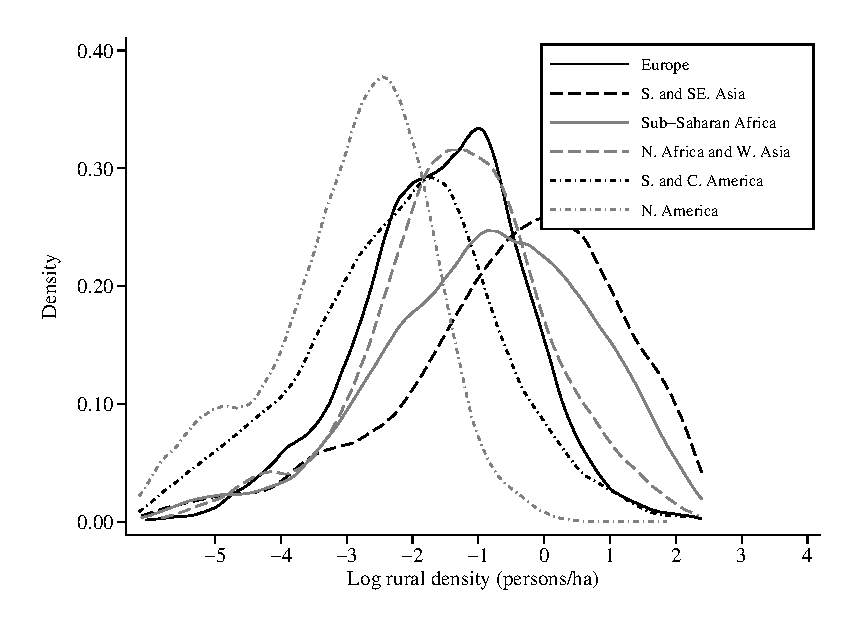
\includegraphics[width=1.0\textwidth]{fig_dens_rurd.eps}
\end{center}
\vspace{-.5cm}\singlespacing {\footnotesize \textbf{Notes}: Kernel density plot, Epanechnikov kernel, of the (log) rural labor/land, $L_{Aisc}/X_{isc}$, at the district level, calculated by the authors using data from \citet{GRUMP} for rural population. ``Temperate'' includes districts that are suitable for growing barley, buckwheat, oats, rye, wheat, and white potatoes, but have zero suitability for cassava, cowpeas, pearl millet, sweet potato, wet rice, and yams. ``Tropical'' includes districts suitable for the latter set of crops, but zero suitability for the former. 
}
\end{figure}

\clearpage

\begin{figure}[!htb]
\begin{center}
\caption{Density Plot of Caloric Yield ($A^{GAEZ}_{is}$), by Crop Type}
\label{FIG_dens_csi}
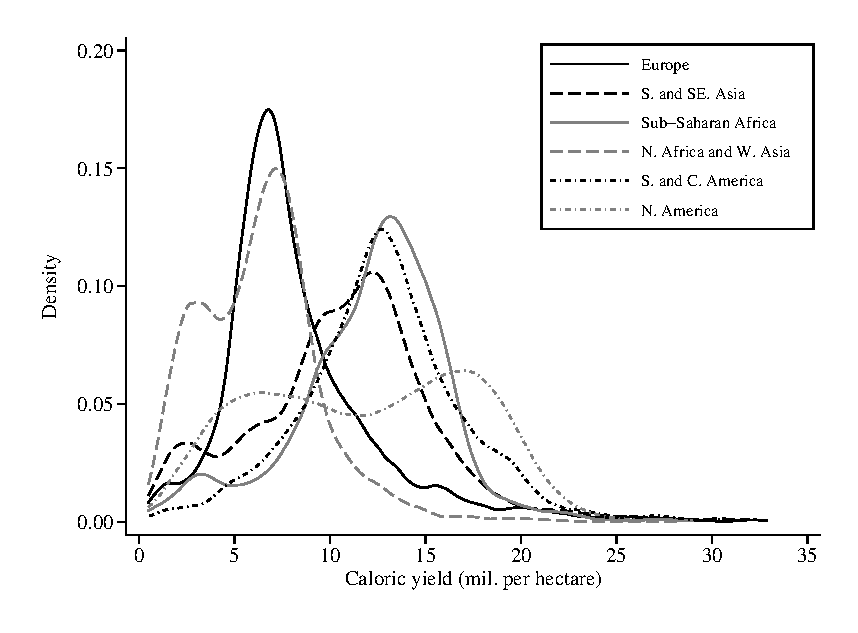
\includegraphics[width=1.0\textwidth]{fig_dens_csi.eps}
\end{center}
\vspace{-.5cm}\singlespacing {\footnotesize \textbf{Notes}: Kernel density plot, Epanechnikov kernel, of the caloric yield, $A_{isc}$, at the district level, calculated by the authors using data from \citet{galorozak2016}. See text for details. This measure sums the maximum calories available per grid cell within a district, then divides by total area of the district. ``Temperate'' includes districts that are suitable for growing barley, buckwheat, oats, rye, wheat, and white potatoes, but have zero suitability for cassava, cowpeas, pearl millet, sweet potato, wet rice, and yams. ``Tropical'' includes districts suitable for the latter set of crops, but zero suitability for the former. 
}
\end{figure}

\clearpage

\begin{figure}[!htb]
\begin{center}
\caption{Residual Relationship of Caloric Yield ($A^{GAEZ}_{is}$) and Rural Labor/Land Ratios}
\label{FIG_beta_crop}
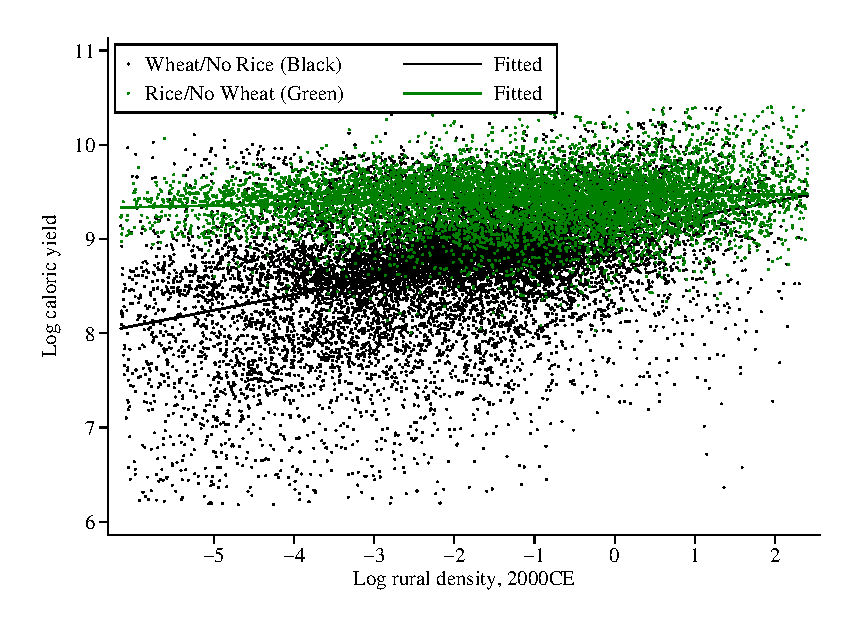
\includegraphics[width=1.0\textwidth]{fig_beta_crop.eps}
\end{center}
\vspace{-.5cm}\singlespacing {\footnotesize \textbf{Notes}: Plotted are the quantile averages of both log caloric yield and log rural labor/land for each sample, temperate and tropical. 50 quantiles are used in each sample. The quantiles are taken from the residuals of caloric yield and rural labor/land after controlling for log light density, urban percentage in 2000, log total population, distance to a city of 100,000 people, road density (km per square kilometers), percent of roads as highways, primary, and secondary roads, the (log) slope and state fixed effects. Linear fits are shown, and the estimated slopes are in the legend. The \texttt{binscatter} command from Stata was used to prepare the figure. ``Temperate'' includes districts that are suitable for growing barley, buckwheat, oats, rye, wheat, and white potatoes, but have zero suitability for cassava, cowpeas, pearl millet, sweet potato, wet rice, and yams. ``Tropical'' includes districts suitable for the latter set of crops, but with zero suitability for the former. 
}
\end{figure}

\clearpage
\begin{table}[!htb]
\begin{center}
\caption{Summary Statistics for District Level Data, 2000CE}
\label{TAB_districts}
{\small
\begin{tabularx}{\textwidth}{lRRRRRRR}
\midrule
 &      &            & \multicolumn{5}{c}{Percentiles:} \\ \cmidrule(lr){4-8}
 & Mean & SD  & 10th    & 25th    & 50th & 75th & 90th \\
\midrule
\multicolumn{8}{l}{Panel A: Population and area} \\ \\
Total population (000s) &    105.8&    480.2&      3.7&      8.4&     22.6&     60.9&    149.1\\
Rural population (000s) &     75.8&    357.5&      3.2&      6.5&     16.0&     40.8&    102.8\\
Urban population (000s) &     29.9&    167.0&      0.0&      0.0&      0.0&     12.9&     52.9\\
Urban share of district pop. &     0.19&     0.27&     0.00&     0.00&     0.00&     0.35&     0.67\\ \\
Share of state population &     0.05&     0.09&     0.00&     0.00&     0.02&     0.06&     0.14\\
Share of state urban pop. &     0.04&     0.13&     0.00&     0.00&     0.00&     0.01&     0.08\\
Share of state area &     0.06&     0.09&     0.00&     0.01&     0.02&     0.07&     0.15\\
\\Total area (000s ha) &    179.8&    475.7&      8.7&     17.1&     53.3&    160.4&    394.5\\
\\
\multicolumn{8}{l}{Panel B: Labor/land ratios, yields, and other controls} \\ \\
Labor/land (persons/ha) &     0.76&     1.19&     0.05&     0.13&     0.34&     0.81&     1.92\\
Caloric yield (mil cals/ha) &    10.83&     4.83&     5.01&     7.20&    10.68&    13.83&    16.93\\
Log light density &    -2.97&     2.92&    -6.43&    -3.93&    -2.63&    -1.03&     0.20\\
Road density (km per sq-km) &     0.40&     0.53&     0.06&     0.11&     0.22&     0.47&     0.90\\
Share of roads, highway &     0.03&     0.09&     0.00&     0.00&     0.00&     0.00&     0.08\\
Share of roads, primary &     0.15&     0.20&     0.00&     0.00&     0.09&     0.22&     0.39\\
Share of roads, secondary &     0.33&     0.30&     0.00&     0.08&     0.24&     0.51&     0.82\\
Slope index &    70.78&    24.18&    33.64&    52.63&    77.69&    91.88&    97.05\\
Distance (km) to city w/ 100,000 &    61.20&    70.57&     6.89&    16.95&    40.33&    78.50&   137.32\\
\midrule
\end{tabularx}
}
\end{center}
\vspace{-.5cm}\singlespacing {\footnotesize \textbf{Notes}: These are summary statistics for districts used in the regression analysis. There are a total of\districts \ observations for each variable (these come from\provinces \ states in\countries \ countries). All population data is derived from GRUMP \citep{GRUMP}. Districts are defined by the \citet{gadm}, and correspond to 2nd-level administrative areas within countries (e.g. counties). Caloric yield, $A^{GAEZ}_{is}$, is calculated by the authors using data from \citet{galorozak2016}. Rural labor/land ratios, $L_{Ais}/X_{is}$, is calculated by the authors using data from \citet{hyde31} for rural population. Both caloric yield and rural labor/land ratios were trimmed at the 99th and 1st percentiles of their raw data prior to calculating the summary statistics in this table. Log mean light density is derived from the Global Radiance Calibrated Nightime Lights data provided by NOAA/NGDC, as in \citet{hssw2016}. Road density and the share of roads by type are from \citet{GRIPS}. The slope index is from \citet{gaez}. Distance from nearest city of 100,000 population is the authors calculation using centroids of districts (see text).
}
\end{table}

\clearpage

\begin{table}[!htb]
\begin{center}
\caption{Summary Statistics on Migration from DHS Surveys}
\label{TAB_migration}
{\small
\begin{tabularx}{\textwidth}{lXXXXXXX}
\midrule
 &      &            & \multicolumn{5}{c}{Percentiles:} \\ \cmidrule{4-8}
 & Mean & SD  & 10th    & 25th    & 50th & 75th & 90th \\
\midrule
\\
\multicolumn{8}{l}{Panel A: Share moving measured by } \\ \\
All movers / all inds. &     0.49&     0.14&     0.32&     0.42&     0.50&     0.59&     0.67\\
Movers in last 5 years / all inds. &     0.21&     0.09&     0.11&     0.15&     0.21&     0.26&     0.33\\
Movers aged 25-50 / all aged 25-50 &     0.54&     0.15&     0.35&     0.43&     0.55&     0.66&     0.73\\
\\
\multicolumn{8}{l}{Panel B: Share of movers to location by self-reported origin:} \\ \\
To urban areas from country &     0.40&     0.15&     0.19&     0.32&     0.41&     0.51&     0.59\\
To rural ares from city or town &     0.17&     0.12&     0.03&     0.07&     0.14&     0.27&     0.35\\
\midrule
\end{tabularx}
}
\end{center}
\vspace{-.5cm}\singlespacing {\footnotesize \textbf{Notes}: This table shows the overall prevalence of migration (Panel A), and the prevalence of migration between different areas (Panel B). These are summary statistics of shares calculated from individual DHS surveys \citep{DHS}. The top panel is based on 86 surveys representing 43 countries. The bottom panel is based on 68 surveys representing 34 countries. 
}
\end{table}

\clearpage

\begin{table}[!htb]
\begin{center}
\caption{Estimates of Land Elasticity, $\beta_g$, by Agricultural Type, 2000CE}
\label{TAB_beta_crops}
{\footnotesize
\begin{tabularx}{\textwidth}{lXXXXXX}
\midrule
\multicolumn{7}{l}{Dependent Variable in all panels: Log caloric yield ($A^{GAEZ}_{isg}$)} \\ \\
\multicolumn{7}{l}{Panel A: Regions defined by:} \\ \\
 & \multicolumn{2}{c}{Crop suitability:} & \multicolumn{2}{c}{Frost Days:} & \multicolumn{2}{c}{Koeppen-Geiger:}\\ \cmidrule(lr){2-3} \cmidrule(lr){4-5} \cmidrule(lr){6-7} 
 & Temperate & Tropical & Temperate  & Tropical  & Temperate  & Tropical \\
 & (1) & (2) & (3) & (4) & (5) & (6) \\
\midrule
Log labor/land ratio ($\beta_g$)&       0.285&       0.126&       0.262&       0.130&       0.272&       0.117\\
                    &     (0.043)&     (0.023)&     (0.044)&     (0.014)&     (0.044)&     (0.019)\\
\midrule
p-value $\beta_g=0$ &       0.000&       0.000&       0.000&       0.000&       0.000&       0.000\\
p-value $\beta_g=\beta_{Temp}$&            &       0.001&            &       0.004&            &       0.001\\
Countries           &          72&          67&          88&          96&          81&          72\\
Observations        &        8416&        6731&       13811&       13879&        9287&        9457\\
R-square (ex. FE)   &        0.19&        0.15&        0.16&        0.13&        0.18&        0.14\\
\midrule
\\
\multicolumn{7}{l}{Panel B: With other restrictions (using crop suitability to define temperate/tropical)} \\ \\
 & \multicolumn{2}{c}{Urban Pop. $<50K$:} & \multicolumn{2}{c}{Pop. share $<0.05$:} & \multicolumn{2}{c}{Ex. Europe/N. Amer.:} \\ \cmidrule(lr){2-3} \cmidrule(lr){4-5} \cmidrule(lr){6-7}
 & Temperate & Tropical & Temperate  & Tropical  & Temperate  & Tropical \\
 & (1) & (2) & (3) & (4) & (5) & (6) \\
\midrule
Log labor/land ratio ($\beta_g$)&       0.300&       0.126&       0.296&       0.124&       0.298&       0.124\\
                    &     (0.045)&     (0.024)&     (0.048)&     (0.025)&     (0.045)&     (0.023)\\
\midrule
p-value $\beta_g=0$ &       0.000&       0.000&       0.000&       0.000&       0.000&       0.000\\
p-value $\beta_g=\beta_{Temp}$&            &       0.001&            &       0.001&            &       0.001\\
Countries           &          68&          66&          56&          36&          17&          62\\
Observations        &        7529&        6192&        6429&        4071&         813&        6676\\
R-square (ex. FE)   &        0.20&        0.16&        0.20&        0.17&        0.15&        0.11\\
\midrule
\end{tabularx}
}
\end{center}
\vspace{-.5cm}\singlespacing {\footnotesize \textbf{Notes}: Conley standard errors, adjusted for spatial auto-correlation with a cutoff distance of 500km, are shown in parentheses. All regressions include state fixed effects, a constant, and controls for the district urbanization rate, log density of district nighttime lights, log total population, log road density, share of roads of different types, distance to nearest city of 100,000 people, and a log slope index. The coefficient estimate on rural population labor/land indicates the value of $\beta_g$, see equation (\ref{EQ_regress}). Rural population is from GRUMP database \citep{grump2011}, and caloric yield is the author's calculations based on the data from \citet{galorozak2016}. Inclusion of districts in the regression is based on the listed criteria, either crop suitability, the number of frost-free days, or K{\"o}ppen-Geiger climate zones. See text for details of how temperate and tropical regions are defined in each case. In Panel B, the columns only include districts with less than 50,000 urban residents, include districts that are less that 5\% of state population, or exclude districts from any country in Europe (incl. Russia east of the Urals) or North America.
}
\end{table}

\clearpage

\begin{table}[!htb]
\begin{center}
\caption{Estimates of Land Elasticity, $\beta_g$, Additional Robustness Checks}
\label{TAB_beta_robust}
{\footnotesize
\begin{tabularx}{\textwidth}{lXXXXXX}
\midrule
\multicolumn{7}{l}{Dependent Variable in all panels: Log caloric yield ($A^{GAEZ}_{isg}$)} \\ \\
\multicolumn{7}{l}{Panel A: Different rural population sources} \\ \\
 & \multicolumn{2}{c}{GRUMP 1990:} & \multicolumn{2}{c}{HYDE 2000:} & \multicolumn{2}{c}{IPUMS (various):}\\ \cmidrule(lr){2-3} \cmidrule(lr){4-5} \cmidrule(lr){6-7} 
 & Temperate & Tropical & Temperate  & Tropical  & Temperate  & Tropical \\
 & (1) & (2) & (3) & (4) & (5) & (6) \\
\midrule
Log labor/land ratio ($\beta_g$)&       0.288&       0.126&       0.241&       0.117&       0.190&       0.017\\
                    &     (0.042)&     (0.023)&     (0.014)&     (0.018)&     (0.087)&     (0.017)\\
\midrule
p-value $\beta_g=0$ &       0.000&       0.000&       0.000&       0.000&       0.029&       0.326\\
p-value $\beta_g=\beta_{Temp}$&            &       0.001&            &       0.000&            &       0.040\\
Countries           &          72&          67&          72&          68&          22&          24\\
Observations        &        8416&        6731&        8170&        6465&        1103&        2416\\
R-square (ex. FE)   &        0.19&        0.15&        0.20&        0.17&        0.08&        0.07\\
\midrule
\\
\multicolumn{7}{l}{Panel B: Different land assumptions (with GRUMP labor/land ratio)} \\ \\
 & \multicolumn{2}{c}{Cultivated Area:} & \multicolumn{2}{c}{Cash crops $<10\%$ area:} & \multicolumn{2}{c}{Pasture $<50\%$ area:}\\ \cmidrule(lr){2-3} \cmidrule(lr){4-5} \cmidrule(lr){6-7}
 & Temperate & Tropical & Temperate  & Tropical  & Temperate  & Tropical \\
 & (1) & (2) & (3) & (4) & (5) & (6) \\
\midrule
Log labor/land ratio ($\beta_g$)&       0.278&       0.126&       0.257&       0.108&       0.286&       0.137\\
                    &     (0.044)&     (0.024)&     (0.050)&     (0.032)&     (0.044)&     (0.025)\\
\midrule
p-value $\beta_g=0$ &       0.000&       0.000&       0.000&       0.001&       0.000&       0.000\\
p-value $\beta_g=\beta_{Temp}$&            &       0.002&            &       0.011&            &       0.003\\
Countries           &          72&          66&          55&          37&          70&          64\\
Observations        &        8382&        6694&        5679&        2356&        7582&        5692\\
R-square (ex. FE)   &        0.18&        0.14&        0.18&        0.15&        0.19&        0.16\\
\midrule
\end{tabularx}
}
\end{center}
\vspace{-.5cm}\singlespacing {\footnotesize \textbf{Notes}: Temperate and tropical samples are defined by the suitability measures described in Table \ref{TAB_beta_crops}. Conley standard errors, adjusted for spatial auto-correlation with a cutoff distance of 500km, are shown in parentheses. All regressions include state fixed effects, a constant, and controls for the district urbanization rate, log density of district nighttime lights, log total population, log road density, share of roads of different types, distance to nearest city of 100,000 people, and a log slope index. The coefficient estimate on rural population labor/land indicates the value of $\beta_g$, see equation (\ref{EQ_regress}). Caloric yield is the author's calculations based on the data from \citet{galorozak2016}. In Panel A, the population data used to define rural labor/land differs based on the heading in the table (see text for details). In Panel B, the first set of results use rural population (from GRUMP) relative to cultivated land area (as opposed to actual land area) to measure labor/land ratios. The second set drops districts that have less than 10\% of their area in cash crops (see text for list of those crops), and the third set shows results for districts that have less than 50\% of their area as pasture land.
}
\end{table}

\clearpage

\begin{table}[!htb]
\begin{center}
\caption{Estimates of Land Elasticity, $\beta_g$, Alternative Productivity Measures}
\label{TAB_beta_prod}
{\footnotesize
\begin{tabularx}{\textwidth}{lXXXXXX}
\midrule
\multicolumn{7}{l}{Dependent Variable in all panels: Log caloric yield ($A^{GAEZ}_{isg}$)} \\ \\
\multicolumn{7}{l}{Panel A: Caloric yield based on GAEZ input/water use:} \\ \\
 & \multicolumn{2}{c}{Medium/Irrigated:} & \multicolumn{2}{c}{High/Rain-fed:} & \multicolumn{2}{c}{High/Irrigated:}\\ \cmidrule(lr){2-3} \cmidrule(lr){4-5} \cmidrule(lr){6-7} 
 & Temperate & Tropical & Temperate  & Tropical  & Temperate  & Tropical \\
 & (1) & (2) & (3) & (4) & (5) & (6) \\
\midrule
Log labor/land ratio ($\beta_g$)&       0.254&       0.120&       0.286&       0.132&       0.253&       0.120\\
                    &     (0.050)&     (0.022)&     (0.045)&     (0.025)&     (0.050)&     (0.022)\\
\midrule
p-value $\beta_g=0$ &       0.000&       0.000&       0.000&       0.000&       0.000&       0.000\\
p-value $\beta_g=\beta_{Temp}$&            &       0.014&            &       0.003&            &       0.014\\
Countries           &          72&          67&          72&          67&          72&          67\\
Observations        &        8416&        6731&        8389&        6719&        8416&        6731\\
R-square (ex. FE)   &        0.17&        0.14&        0.18&        0.14&        0.17&        0.14\\
\midrule
\end{tabularx}
}
\end{center}
\vspace{-.5cm}\singlespacing {\footnotesize \textbf{Notes}: Temperate and tropical samples are defined by the suitability measures described in Table \ref{TAB_beta_crops}. Conley standard errors, adjusted for spatial auto-correlation with a cutoff distance of 500km, are shown in parentheses. All regressions include state fixed effects, a constant, and controls for the district urbanization rate, log density of district nighttime lights, log total population, log road density, share of roads of different types, distance to nearest city of 100,000 people, and a log slope index. The coefficient estimate on rural population labor/land indicates the value of $\beta_g$, see equation (\ref{EQ_regress}). In Panel A, the construction of the $A^{GAEZ}_{isg}$ caloric suitability yield differs across the columns. In (1) and (2), the yield is derived from the underlying GAEZ medium input-irrigated data, and the following columns use the high input, rain-fed data, or the high input, irrigated data, as noted. 
}
\end{table}


\begin{table}[!htb]
\begin{center}
\caption{Estimates of Land Elasticity, $\beta_g$, with DHS district controls}
\label{TAB_beta_dhs}
{\footnotesize
\begin{tabularx}{\textwidth}{lXXXXXX}
\midrule
\multicolumn{7}{l}{Dependent Variable in all columns: Log caloric yield ($A^{GAEZ}_{isg}$)} \\ \\
 & Temperate & Tropical & Temperate  & Tropical  & Temperate  & Tropical \\
 & (1) & (2) & (3) & (4) & (5) & (6) \\
\midrule
Log labor/land ratio ($\beta_g$)   &       0.375&       0.104&       0.375&       0.102&       0.374&       0.110\\
                    &     (0.081)&     (0.020)&     (0.080)&     (0.020)&     (0.083)&     (0.021)\\
Demog. controls     &          No&          No&         Yes&         Yes&         Yes&         Yes\\
Asset controls      &          No&          No&          No&          No&         Yes&         Yes\\
\midrule
p-value $\beta_g=0$ &       0.000&       0.000&       0.000&       0.000&       0.000&       0.000\\
p-value $\beta_g=\beta_{Temp}$&            &       0.000&            &       0.000&            &       0.000\\
Countries           &          15&          29&          15&          29&          15&          29\\
Observations        &         290&        1291&         290&        1291&         290&        1291\\
R-square            &        0.82&        0.82&        0.82&        0.82&        0.83&        0.82\\
\midrule
\end{tabularx}
}
\end{center}
\vspace{-.5cm}\singlespacing {\footnotesize \textbf{Notes}: Temperate and tropical samples are defined by the suitability measures described in Table \ref{TAB_beta_crops}. Conley standard errors, adjusted for spatial auto-correlation with a cutoff distance of 500km, are shown in parentheses. All regressions include state fixed effects, a constant, and controls for the district urbanization rate, log density of district nighttime lights, log total population, log road density, share of roads of different types, distance to nearest city of 100,000 people, and a log slope index. The coefficient estimate on rural population labor/land indicates the value of $\beta_g$, see equation (\ref{EQ_regress}). The districts included in these regressions have villages/clusters that took part in a Demographic and Health Survey (DHS). Using the DHS data, the columns include district level means or medians of demograhpic variables (e.g. household head education and age) and asset variables (e.g. household ownership of cattle or use of electricity), see text for details of the precise controls.
}
\end{table}

\clearpage

\begin{table}[!htb]
\begin{center}
\caption{Estimates of Land Elasticity, $\beta_g$, for Mixed Region, 2000CE}
\label{TAB_beta_mixed}
{\footnotesize
\begin{tabularx}{\textwidth}{lXXXXXX}
\midrule
\multicolumn{7}{l}{Dependent variable: Log caloric yield ($A^{GAEZ}_{isg}$)} \\ \\
 & \multicolumn{6}{c}{Specification defined by:} \\ \cmidrule(lr){2-7} 
 &          &  Urban Pop. & Ex. Europe    & Land $X_{is}$    & Cash crops  & GAEZ  \\
 & Baseline &$<50K$       & N. Amer. & cult. area       & $<10\%$ area &  high Input \\
 & (1) & (2) & (3) & (4) & (5) & (6) \\
\midrule
Log labor/land ratio ($\beta_g$)&       0.167&       0.175&       0.121&       0.164&       0.183&       0.176\\
                    &     (0.022)&     (0.024)&     (0.016)&     (0.023)&     (0.030)&     (0.024)\\
\midrule
p-value $\beta_g=0$ &       0.000&       0.000&       0.000&       0.000&       0.000&       0.000\\
p-value $\beta_g=\beta_g^{Temp}$&       0.001&       0.001&       0.005&       0.002&       0.111&       0.005\\
p-value $\beta_g=\beta_g^{Trop}$&       0.155&       0.111&       0.975&       0.183&       0.104&       0.143\\
Countries           &         106&          99&          55&         105&          71&         105\\
Observations        &       12388&       10800&        6301&       12342&        6010&       12321\\
R-square (ex. FE)   &        0.13&        0.13&        0.09&        0.12&        0.14&        0.11\\
\midrule
\end{tabularx}
}
\end{center}
\vspace{-.5cm}\singlespacing {\footnotesize \textbf{Notes}: For all regressions, the sample includes districts that are suitable for both temperate and tropical crops, as defined in the text. Conley standard errors, adjusted for spatial auto-correlation with a cutoff distance of 500km, are shown in parentheses. All regressions include state fixed effects, a constant, and controls for the district urbanization rate, log density of district nighttime lights, log total population, log road density, share of roads of different types, distance to nearest city of 50,000 people, and a log slope index. The coefficient estimate on rural population labor/land indicates the value of $\beta_g$, see equation (\ref{EQ_regress}). Rural population is from GRUMP database \citep{grump2011}, and caloric yield is the author's calculations based on the data from \citet{galorozak2016}. Inclusion of districts in the regression is based on the listed criteria. Column (4) uses cultivated land (rather than total land) to measure the labor/land ratio. Column (5) excludes districts that have more than 10\% of their total land used for cash crops. Column (6) measures the caloric yield with the GAEZ high input measure of agricultural potential (as opposed to the low input baseline).
}
\end{table}

\clearpage
\begin{table}[!htb]
\begin{center}
\caption{Country-level aggregate land elasticity estimates}
\label{TAB_beta_country}
{\footnotesize
\begin{tabularx}{\textwidth}{lXlXlXlX}
\midrule
Country & $\beta$ & Country & $\beta$ & Country & $\beta$ & Country & $\beta$ \\
\midrule
Afghanistan &     0.202 & Egypt &     0.173 & Lithuania &     0.285 & Sao Tome &     0.133 \\
Albania &     0.180 & El Salvador &     0.129 & Luxembourg &     0.285 & Senegal &     0.126 \\
Algeria &     0.212 & Eq. Guinea &     0.128 & Macao &     0.167 & Serbia &     0.202 \\
American Samoa &     0.126 & Eritrea &     0.153 & Madagascar &     0.165 & Sierra Leone &     0.133 \\
Angola &     0.165 & Estonia &     0.285 & Malawi &     0.161 & Slovakia &     0.274 \\
Argentina &     0.179 & Ethiopia &     0.164 & Malaysia &     0.137 & Slovenia &     0.276 \\
Australia &     0.176 & Fiji &     0.145 & Mali &     0.126 & Solomon Islands &     0.125 \\
Austria &     0.285 & Finland &     0.285 & Martinique &     0.126 & Somalia &     0.132 \\
Azerbaijan &     0.183 & France &     0.245 & Mauritania &     0.133 & South Africa &     0.167 \\
Bangladesh &     0.166 & French Guiana &     0.126 & Mexico &     0.165 & South Korea &     0.189 \\
Belarus &     0.285 & Gabon &     0.126 & Mongolia &     0.285 & South Sudan &     0.128 \\
Belgium &     0.285 & Gambia &     0.126 & Morocco &     0.171 & Spain &     0.177 \\
Benin &     0.126 & Georgia &     0.188 & Mozambique &     0.159 & Sri Lanka &     0.128 \\
Bhutan &     0.205 & Germany &     0.285 & Myanmar &     0.161 & Sudan &     0.134 \\
Bolivia &     0.157 & Ghana &     0.126 & Namibia &     0.167 & Suriname &     0.126 \\
Bosnia &     0.197 & Greece &     0.167 & Netherlands &     0.285 & Swaziland &     0.171 \\
Botswana &     0.167 & Guadeloupe &     0.126 & New Caledonia &     0.164 & Sweden &     0.285 \\
Brazil &     0.140 & Guatemala &     0.157 & New Zealand &     0.279 & Switzerland &     0.281 \\
Brunei &     0.126 & Guinea &     0.139 & Nicaragua &     0.131 & Syria &     0.200 \\
Bulgaria &     0.204 & Guinea-Bissau &     0.126 & Niger &     0.131 & Taiwan &     0.167 \\
Burkina Faso &     0.126 & Guyana &     0.134 & Nigeria &     0.128 & Tajikistan &     0.198 \\
Burundi &     0.181 & Haiti &     0.142 & North Korea &     0.266 & Tanzania &     0.157 \\
C. African Rep. &     0.126 & Honduras &     0.151 & Norway &     0.285 & Thailand &     0.138 \\
Cambodia &     0.128 & Hungary &     0.213 & Oman &     0.172 & Timor-Leste &     0.129 \\
Cameroon &     0.139 & India &     0.157 & Pakistan &     0.170 & Togo &     0.126 \\
Canada &     0.283 & Indonesia &     0.141 & Palestina &     0.182 & Tunisia &     0.167 \\
Chad &     0.127 & Iran &     0.195 & Panama &     0.134 & Turkey &     0.218 \\
Chile &     0.260 & Iraq &     0.172 & Papau N.G. &     0.154 & Uganda &     0.141 \\
China &     0.173 & Isle of Man &     0.285 & Paraguay &     0.165 & Ukraine &     0.278 \\
Colombia &     0.141 & Italy &     0.167 & Peru &     0.156 & United Kingdom &     0.284 \\
Costa Rica &     0.145 & Japan &     0.192 & Philippines &     0.131 & United States &     0.203 \\
Cote d'Ivoire &     0.126 & Jordan &     0.239 & Poland &     0.285 & Uruguay &     0.167 \\
Croatia &     0.212 & Kazakhstan &     0.280 & Portugal &     0.178 & Uzbekistan &     0.251 \\
Cuba &     0.128 & Kenya &     0.157 & Rep. of Congo &     0.127 & Vanuatu &     0.130 \\
Czech Republic &     0.285 & Kosovo &     0.247 & Reunion &     0.169 & Venezuela &     0.145 \\
D.R. Congo &     0.141 & Kyrgyzstan &     0.275 & Romania &     0.243 & Vietnam &     0.154 \\
Denmark &     0.285 & Laos &     0.160 & Russia &     0.278 & Virgin Islands, U.S. &     0.126 \\
Djibouti &     0.126 & Latvia &     0.285 & Rwanda &     0.210 & Zambia &     0.167 \\
Dominican Rep. &     0.144 & Lebanon &     0.184 & Samoa &     0.132 & Zimbabwe &     0.167 \\
Ecuador &     0.159&Liberia &     0.126 & & & & \\
\midrule
\end{tabularx}
}
\end{center}
\vspace{-.5cm}\singlespacing {\footnotesize \textbf{Notes}: This table reports the aggregated value of the land elasticity, $\beta$, for each country. The aggregate value is a weighted average of district land elasticities with tropical districts (0.125), temperate districts (0.287), and mixed districts (0.168) that can grow both tropical and temperate crops. The weights in the average are the maximum calories that can be produced in a district relative to the maximum calories that can be produced by all districts in the country. 
}
\end{table}

\clearpage
\begin{table}[!htb]
\begin{center}
\caption{Panel Estimates of Effect of Population Change, by Land Elasticity}
\label{TAB_pop_panel}
{\footnotesize
\begin{tabularx}{\textwidth}{lXXXXXX}
\midrule
 & \multicolumn{6}{c}{Dependent Variable:} \\ \cmidrule(lr){2-7}
 & \multicolumn{2}{c}{Log GDP per capita} & \multicolumn{2}{c}{Log GDP per worker} & \multicolumn{2}{c}{Log population} \\ \cmidrule(lr){2-3} \cmidrule(lr){4-5} \cmidrule(lr){6-7}
 & Tropical & Temperate & Tropical & Temperate & Tropical & Temperate \\
 & (1) & (2) & (3) & (4) & (5) & (6) \\
\midrule
 & \multicolumn{6}{c}{Panel A:} \\ \cmidrule(lr){2-7}
Mortality rate      &       0.403&       1.226&       0.418&       1.273&      -0.255&      -1.442\\
                    &     (0.151)&     (0.132)&     (0.158)&     (0.140)&     (0.108)&     (0.193)\\
\midrule
p-value $\theta=0$  &       0.008&       0.000&       0.009&       0.000&       0.019&       0.000\\
p-value $\theta=\theta^{Trop}$&           .&       0.000&           .&       0.000&           .&       0.000\\
Countries           &          30&           5&          30&           5&          30&           5\\
Observations        &         238&          40&         238&          40&         238&          40\\
\midrule
\\
 & \multicolumn{6}{c}{Panel B:} \\ \cmidrule(lr){2-7}
Log life expectancy &      -0.743&      -2.180&      -0.703&      -2.324&       1.383&       2.870\\
                    &     (0.290)&     (0.171)&     (0.285)&     (0.187)&     (0.165)&     (0.248)\\
\midrule
p-value $\theta=0$  &       0.011&       0.000&       0.014&       0.000&       0.000&       0.000\\
p-value $\theta=\theta^{Below}$&           .&       0.000&           .&       0.000&           .&       0.000\\
Countries           &          30&           5&          30&           5&          30&           5\\
Observations        &         224&          40&         224&          40&         224&          40\\
\midrule
\end{tabularx}
}
\end{center}
\vspace{-.5cm}\singlespacing {\footnotesize \textbf{Notes}: Robust standard errors are reported in parentheses. All regressions include both year fixed effects and country fixed effects. Countries are assigned as either ``Temperate'' or ``Tropical'' based on their estimated $\beta$ from Table \ref{TAB_beta_country}. Those with $\beta<0.20$ are classified as tropical, while those with $\beta>=0.20$ are classified as temperate. The mortality rate used as an explanatory variable in Panel A is the mortality rate from 15 infectious diseases, as documented by \cite{aj07}. All data on GDP per capita, GDP per worker, population, and life expectancy is also taken from those author's dataset. The p-value of $\theta = \theta^{Trop}$ is from a test that the estimated coefficient for temperate countries is identical to the estimated coefficient of tropical countries.
}
\end{table}



\end{document}